\documentclass[twoside]{book}

% Packages required by doxygen
\usepackage{fixltx2e}
\usepackage{calc}
\usepackage{doxygen}
\usepackage[export]{adjustbox} % also loads graphicx
\usepackage{graphicx}
\usepackage[utf8]{inputenc}
\usepackage{makeidx}
\usepackage{multicol}
\usepackage{multirow}
\PassOptionsToPackage{warn}{textcomp}
\usepackage{textcomp}
\usepackage[nointegrals]{wasysym}
\usepackage[table]{xcolor}

% Font selection
\usepackage[T1]{fontenc}
\usepackage[scaled=.90]{helvet}
\usepackage{courier}
\usepackage{amssymb}
\usepackage{sectsty}
\renewcommand{\familydefault}{\sfdefault}
\allsectionsfont{%
  \fontseries{bc}\selectfont%
  \color{darkgray}%
}
\renewcommand{\DoxyLabelFont}{%
  \fontseries{bc}\selectfont%
  \color{darkgray}%
}
\newcommand{\+}{\discretionary{\mbox{\scriptsize$\hookleftarrow$}}{}{}}

% Page & text layout
\usepackage{geometry}
\geometry{%
  a4paper,%
  top=2.5cm,%
  bottom=2.5cm,%
  left=2.5cm,%
  right=2.5cm%
}
\tolerance=750
\hfuzz=15pt
\hbadness=750
\setlength{\emergencystretch}{15pt}
\setlength{\parindent}{0cm}
\setlength{\parskip}{3ex plus 2ex minus 2ex}
\makeatletter
\renewcommand{\paragraph}{%
  \@startsection{paragraph}{4}{0ex}{-1.0ex}{1.0ex}{%
    \normalfont\normalsize\bfseries\SS@parafont%
  }%
}
\renewcommand{\subparagraph}{%
  \@startsection{subparagraph}{5}{0ex}{-1.0ex}{1.0ex}{%
    \normalfont\normalsize\bfseries\SS@subparafont%
  }%
}
\makeatother

% Headers & footers
\usepackage{fancyhdr}
\pagestyle{fancyplain}
\fancyhead[LE]{\fancyplain{}{\bfseries\thepage}}
\fancyhead[CE]{\fancyplain{}{}}
\fancyhead[RE]{\fancyplain{}{\bfseries\leftmark}}
\fancyhead[LO]{\fancyplain{}{\bfseries\rightmark}}
\fancyhead[CO]{\fancyplain{}{}}
\fancyhead[RO]{\fancyplain{}{\bfseries\thepage}}
\fancyfoot[LE]{\fancyplain{}{}}
\fancyfoot[CE]{\fancyplain{}{}}
\fancyfoot[RE]{\fancyplain{}{\bfseries\scriptsize Generated by Doxygen }}
\fancyfoot[LO]{\fancyplain{}{\bfseries\scriptsize Generated by Doxygen }}
\fancyfoot[CO]{\fancyplain{}{}}
\fancyfoot[RO]{\fancyplain{}{}}
\renewcommand{\footrulewidth}{0.4pt}
\renewcommand{\chaptermark}[1]{%
  \markboth{#1}{}%
}
\renewcommand{\sectionmark}[1]{%
  \markright{\thesection\ #1}%
}

% Indices & bibliography
\usepackage{natbib}
\usepackage[titles]{tocloft}
\setcounter{tocdepth}{3}
\setcounter{secnumdepth}{5}
\makeindex

% Hyperlinks (required, but should be loaded last)
\usepackage{ifpdf}
\ifpdf
  \usepackage[pdftex,pagebackref=true]{hyperref}
\else
  \usepackage[ps2pdf,pagebackref=true]{hyperref}
\fi
\hypersetup{%
  colorlinks=true,%
  linkcolor=blue,%
  citecolor=blue,%
  unicode%
}

% Custom commands
\newcommand{\clearemptydoublepage}{%
  \newpage{\pagestyle{empty}\cleardoublepage}%
}

\usepackage{caption}
\captionsetup{labelsep=space,justification=centering,font={bf},singlelinecheck=off,skip=4pt,position=top}

%===== C O N T E N T S =====

\begin{document}

% Titlepage & ToC
\hypersetup{pageanchor=false,
             bookmarksnumbered=true,
             pdfencoding=unicode
            }
\pagenumbering{alph}
\begin{titlepage}
\vspace*{7cm}
\begin{center}%
{\Large Proyecto final alse }\\
\vspace*{1cm}
{\large Generated by Doxygen 1.8.13}\\
\end{center}
\end{titlepage}
\clearemptydoublepage
\pagenumbering{roman}
\tableofcontents
\clearemptydoublepage
\pagenumbering{arabic}
\hypersetup{pageanchor=true}

%--- Begin generated contents ---
\chapter{Namespace Index}
\section{Namespace List}
Here is a list of all documented namespaces with brief descriptions\+:\begin{DoxyCompactList}
\item\contentsline{section}{\hyperlink{namespace_q_main_window}{Q\+Main\+Window} \\*Esta clase maneja la venta principal que es la primera que vemos al abrir la aplicación }{\pageref{namespace_q_main_window}}{}
\item\contentsline{section}{\hyperlink{namespace_q_string}{Q\+String} \\*Es un tipo de variable que nos permite usar los valores que ingresamos en las ventanas de Qt }{\pageref{namespace_q_string}}{}
\item\contentsline{section}{\hyperlink{namespaceui}{ui} }{\pageref{namespaceui}}{}
\end{DoxyCompactList}

\chapter{Hierarchical Index}
\section{Class Hierarchy}
This inheritance list is sorted roughly, but not completely, alphabetically\+:\begin{DoxyCompactList}
\item \contentsline{section}{db\+\_\+local}{\pageref{classdb__local}}{}
\item Q\+Dialog\begin{DoxyCompactList}
\item \contentsline{section}{aciertos}{\pageref{classaciertos}}{}
\item \contentsline{section}{menu}{\pageref{classmenu}}{}
\item \contentsline{section}{paciente}{\pageref{classpaciente}}{}
\item \contentsline{section}{prueba}{\pageref{classprueba}}{}
\item \contentsline{section}{regpc}{\pageref{classregpc}}{}
\item \contentsline{section}{regu}{\pageref{classregu}}{}
\item \contentsline{section}{tiempod}{\pageref{classtiempod}}{}
\end{DoxyCompactList}
\item Q\+Main\+Window\begin{DoxyCompactList}
\item \contentsline{section}{usuario}{\pageref{classusuario}}{}
\end{DoxyCompactList}
\end{DoxyCompactList}

\chapter{Class Index}
\section{Class List}
Here are the classes, structs, unions and interfaces with brief descriptions\+:\begin{DoxyCompactList}
\item\contentsline{section}{\hyperlink{classaciertos}{aciertos} \\*Esta clase maneja la conexión con la ventana de diálogo que nos muestra los aciertos que tuvo el paciente en la prueba }{\pageref{classaciertos}}{}
\item\contentsline{section}{\hyperlink{classdb__local}{db\+\_\+local} \\*The db\+\_\+\+Local class Esta clase maneja la conexión con la bases de datos en S\+Q\+Lite3 para almacenar permanentemente los datos en un archivo }{\pageref{classdb__local}}{}
\item\contentsline{section}{\hyperlink{classmenu}{menu} \\*Esta clase maneja la conexión con la ventana de diálogo que nos permite elegir entre ingresar un paciente para hacerle la prueba de agilidad o registrar uno nuevo }{\pageref{classmenu}}{}
\item\contentsline{section}{\hyperlink{classpaciente}{paciente} \\*Esta clase maneja la verificación de un paciente en la base de datos }{\pageref{classpaciente}}{}
\item\contentsline{section}{\hyperlink{classprueba}{prueba} \\*Esta clase maneja la ventana de la prueba de agilidad para el paciente }{\pageref{classprueba}}{}
\item\contentsline{section}{\hyperlink{classregpc}{regpc} \\*Esta clase maneja la conexión con la ventana de dialogo Q\+Dialog donde se registran los datos de un paciente nuevo }{\pageref{classregpc}}{}
\item\contentsline{section}{\hyperlink{classregu}{regu} \\*Esta clase denominada regu maneja la conexión con la ventana de dialogo donde se registran los datos de un usuario nuevo }{\pageref{classregu}}{}
\item\contentsline{section}{\hyperlink{classtiempod}{tiempod} \\*Esta clase maneja la conexion con al ventana donde le preguntaremos al usuario la duracion de la prueba de agilidad para el paciente }{\pageref{classtiempod}}{}
\item\contentsline{section}{\hyperlink{classusuario}{usuario} \\*Esta clase maneja la verificacion de usuario que se realiza en la ventana principal }{\pageref{classusuario}}{}
\end{DoxyCompactList}

\chapter{Namespace Documentation}
\hypertarget{namespace_q_main_window}{}\section{Q\+Main\+Window Namespace Reference}
\label{namespace_q_main_window}\index{Q\+Main\+Window@{Q\+Main\+Window}}


Esta clase maneja la venta principal que es la primera que vemos al abrir la aplicación.  




\subsection{Detailed Description}
Esta clase maneja la venta principal que es la primera que vemos al abrir la aplicación. 
\hypertarget{namespace_q_string}{}\section{Q\+String Namespace Reference}
\label{namespace_q_string}\index{Q\+String@{Q\+String}}


es un tipo de variable que nos permite usar los valores que ingresamos en las ventanas de Qt.  




\subsection{Detailed Description}
es un tipo de variable que nos permite usar los valores que ingresamos en las ventanas de Qt. 
\hypertarget{namespaceui}{}\section{ui Namespace Reference}
\label{namespaceui}\index{ui@{ui}}


\subsection{Detailed Description}
\begin{DoxyAuthor}{Authors}
keisy aleman y jeisson velandia 
\end{DoxyAuthor}

\chapter{Class Documentation}
\hypertarget{classaciertos}{}\section{aciertos Class Reference}
\label{classaciertos}\index{aciertos@{aciertos}}


Esta clase maneja la conexión con la ventana de diálogo que nos muestra los aciertos que tuvo el paciente en la prueba .  




{\ttfamily \#include $<$aciertos.\+h$>$}

Inheritance diagram for aciertos\+:\begin{figure}[H]
\begin{center}
\leavevmode
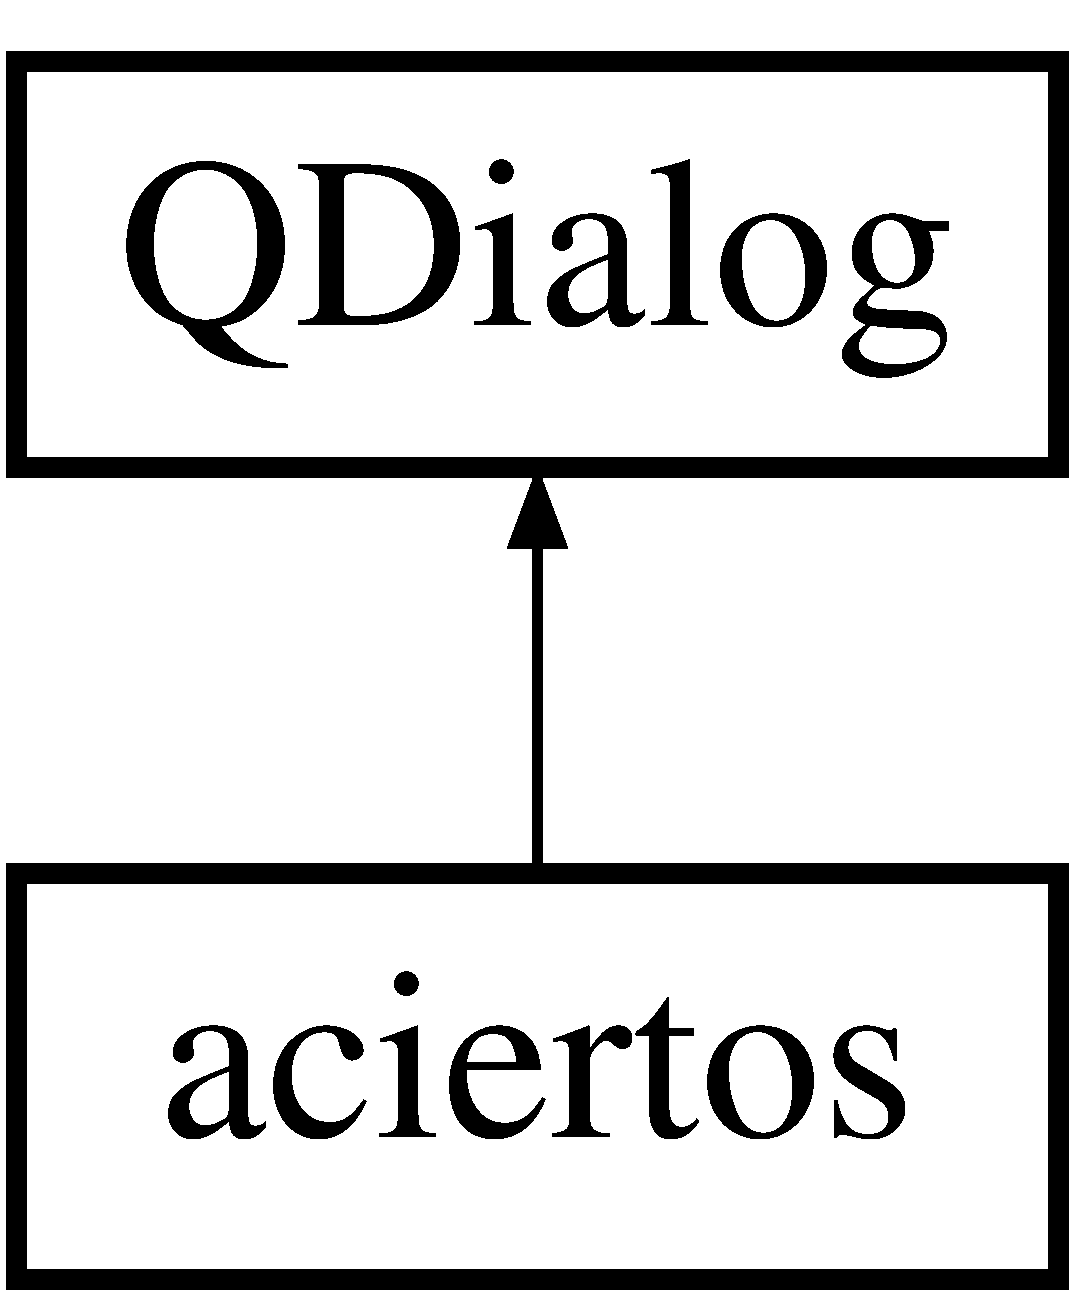
\includegraphics[height=2.000000cm]{classaciertos}
\end{center}
\end{figure}
\subsection*{Public Slots}
\begin{DoxyCompactItemize}
\item 
void \hyperlink{classaciertos_aae3c1efb76360acfff0e058b6ba6ec33}{on\+\_\+volvermenu\+\_\+clicked} ()
\begin{DoxyCompactList}\small\item\em \hyperlink{classaciertos_aae3c1efb76360acfff0e058b6ba6ec33}{aciertos\+::on\+\_\+volvermenu\+\_\+clicked} \end{DoxyCompactList}\item 
void \hyperlink{classaciertos_a1b36eb2a2c3fef95390943d8dacf915d}{on\+\_\+salir\+\_\+clicked} ()
\begin{DoxyCompactList}\small\item\em \hyperlink{classaciertos_a1b36eb2a2c3fef95390943d8dacf915d}{aciertos\+::on\+\_\+salir\+\_\+clicked} \end{DoxyCompactList}\end{DoxyCompactItemize}
\subsection*{Public Member Functions}
\begin{DoxyCompactItemize}
\item 
\hyperlink{classaciertos_a46e28661870e72ccb00b558478420f64}{aciertos} (Q\+Widget $\ast$parent=0)
\begin{DoxyCompactList}\small\item\em \hyperlink{classaciertos_a46e28661870e72ccb00b558478420f64}{aciertos\+::aciertos} Es la función del constructor de la clase aciertos, en este controlamos lo que pasa al abrirse la ventana. \end{DoxyCompactList}\item 
\hyperlink{classaciertos_aef1c2b79f77ef192dd48a2359c78b83d}{$\sim$aciertos} ()
\begin{DoxyCompactList}\small\item\em \hyperlink{classaciertos_aef1c2b79f77ef192dd48a2359c78b83d}{aciertos\+::$\sim$aciertos} Es la función del destructor que controla lo que pasa al cerrarse la ventana. \end{DoxyCompactList}\end{DoxyCompactItemize}


\subsection{Detailed Description}
Esta clase maneja la conexión con la ventana de diálogo que nos muestra los aciertos que tuvo el paciente en la prueba . 

\subsection{Constructor \& Destructor Documentation}
\mbox{\Hypertarget{classaciertos_a46e28661870e72ccb00b558478420f64}\label{classaciertos_a46e28661870e72ccb00b558478420f64}} 
\index{aciertos@{aciertos}!aciertos@{aciertos}}
\index{aciertos@{aciertos}!aciertos@{aciertos}}
\subsubsection{\texorpdfstring{aciertos()}{aciertos()}}
{\footnotesize\ttfamily aciertos\+::aciertos (\begin{DoxyParamCaption}\item[{Q\+Widget $\ast$}]{parent = {\ttfamily 0} }\end{DoxyParamCaption})\hspace{0.3cm}{\ttfamily [explicit]}}



\hyperlink{classaciertos_a46e28661870e72ccb00b558478420f64}{aciertos\+::aciertos} Es la función del constructor de la clase aciertos, en este controlamos lo que pasa al abrirse la ventana. 

EL constructor de la clase.


\begin{DoxyParams}{Parameters}
{\em parent} & es un puntero de tipo Q\+Widget. \\
\hline
\end{DoxyParams}
\mbox{\Hypertarget{classaciertos_aef1c2b79f77ef192dd48a2359c78b83d}\label{classaciertos_aef1c2b79f77ef192dd48a2359c78b83d}} 
\index{aciertos@{aciertos}!````~aciertos@{$\sim$aciertos}}
\index{````~aciertos@{$\sim$aciertos}!aciertos@{aciertos}}
\subsubsection{\texorpdfstring{$\sim$aciertos()}{~aciertos()}}
{\footnotesize\ttfamily aciertos\+::$\sim$aciertos (\begin{DoxyParamCaption}{ }\end{DoxyParamCaption})}



\hyperlink{classaciertos_aef1c2b79f77ef192dd48a2359c78b83d}{aciertos\+::$\sim$aciertos} Es la función del destructor que controla lo que pasa al cerrarse la ventana. 

EL destructor de la clase. 

\subsection{Member Function Documentation}
\mbox{\Hypertarget{classaciertos_a1b36eb2a2c3fef95390943d8dacf915d}\label{classaciertos_a1b36eb2a2c3fef95390943d8dacf915d}} 
\index{aciertos@{aciertos}!on\+\_\+salir\+\_\+clicked@{on\+\_\+salir\+\_\+clicked}}
\index{on\+\_\+salir\+\_\+clicked@{on\+\_\+salir\+\_\+clicked}!aciertos@{aciertos}}
\subsubsection{\texorpdfstring{on\+\_\+salir\+\_\+clicked}{on\_salir\_clicked}}
{\footnotesize\ttfamily void aciertos\+::on\+\_\+salir\+\_\+clicked (\begin{DoxyParamCaption}{ }\end{DoxyParamCaption})\hspace{0.3cm}{\ttfamily [slot]}}



\hyperlink{classaciertos_a1b36eb2a2c3fef95390943d8dacf915d}{aciertos\+::on\+\_\+salir\+\_\+clicked} 

Esta función es una slot que cierra la ventana al hacer click en el botón de salir, cerrando así, el programa. \mbox{\Hypertarget{classaciertos_aae3c1efb76360acfff0e058b6ba6ec33}\label{classaciertos_aae3c1efb76360acfff0e058b6ba6ec33}} 
\index{aciertos@{aciertos}!on\+\_\+volvermenu\+\_\+clicked@{on\+\_\+volvermenu\+\_\+clicked}}
\index{on\+\_\+volvermenu\+\_\+clicked@{on\+\_\+volvermenu\+\_\+clicked}!aciertos@{aciertos}}
\subsubsection{\texorpdfstring{on\+\_\+volvermenu\+\_\+clicked}{on\_volvermenu\_clicked}}
{\footnotesize\ttfamily void aciertos\+::on\+\_\+volvermenu\+\_\+clicked (\begin{DoxyParamCaption}{ }\end{DoxyParamCaption})\hspace{0.3cm}{\ttfamily [slot]}}



\hyperlink{classaciertos_aae3c1efb76360acfff0e058b6ba6ec33}{aciertos\+::on\+\_\+volvermenu\+\_\+clicked} 

Esta función es una slot que cierra la ventana y nos devuelve a la venta de menu.. 

The documentation for this class was generated from the following files\+:\begin{DoxyCompactItemize}
\item 
/home/alseuser/\+Proecto\+\_\+final\+\_\+alse/\+P\+A/aciertos.\+h\item 
/home/alseuser/\+Proecto\+\_\+final\+\_\+alse/\+P\+A/aciertos.\+cpp\end{DoxyCompactItemize}

\hypertarget{classdb__local}{}\section{db\+\_\+local Class Reference}
\label{classdb__local}\index{db\+\_\+local@{db\+\_\+local}}


The db\+\_\+\+Local class Esta clase maneja la conexión con la bases de datos en S\+Q\+Lite3 para almacenar permanentemente los datos en un archivo.  




{\ttfamily \#include $<$db\+\_\+local.\+h$>$}

\subsection*{Public Member Functions}
\begin{DoxyCompactItemize}
\item 
bool \hyperlink{classdb__local_a64ad8edee1a11c82f5d96bfd10a5fdd3}{abrir\+DB} (string path)
\begin{DoxyCompactList}\small\item\em \hyperlink{classdb__local_a64ad8edee1a11c82f5d96bfd10a5fdd3}{db\+\_\+local\+::abrir\+DB} \end{DoxyCompactList}\item 
bool \hyperlink{classdb__local_a4f93f54ed2cacb6d8c1da7b2039f5ff3}{cargarusuario} (string namenew, string lastnamenew, string fnnew, string docinew, string usernuevo, string contranew)
\begin{DoxyCompactList}\small\item\em \hyperlink{classdb__local_a4f93f54ed2cacb6d8c1da7b2039f5ff3}{db\+\_\+local\+::cargarusuario} \end{DoxyCompactList}\item 
bool \hyperlink{classdb__local_ad208904f698ad775e2a14f9f0220d251}{cargarpaciente} (string np, string appc, string Doc, string fecha, string genero, string raza, string direccion, string nin, int edad)
\begin{DoxyCompactList}\small\item\em \hyperlink{classdb__local_ad208904f698ad775e2a14f9f0220d251}{db\+\_\+local\+::cargarpaciente} \end{DoxyCompactList}\item 
bool \hyperlink{classdb__local_abfb0cb98687cd548429b15e537fbaf2f}{cargardatos} (int docu, int conteo, int \+\_\+estado2, int seg)
\begin{DoxyCompactList}\small\item\em \hyperlink{classdb__local_abfb0cb98687cd548429b15e537fbaf2f}{db\+\_\+local\+::cargardatos} \end{DoxyCompactList}\item 
bool \hyperlink{classdb__local_a54ef2e3aa44fcfb68f9dd02c64ae8421}{verificarusuario} (\hyperlink{classusuario}{usuario} \&z)
\begin{DoxyCompactList}\small\item\em \hyperlink{classdb__local_a54ef2e3aa44fcfb68f9dd02c64ae8421}{db\+\_\+local\+::verificarusuario} \end{DoxyCompactList}\item 
bool \hyperlink{classdb__local_af39c3f536549485b9ec8e614f92870c1}{verificarpaciente} (\hyperlink{classpaciente}{paciente} \&p)
\begin{DoxyCompactList}\small\item\em \hyperlink{classdb__local_af39c3f536549485b9ec8e614f92870c1}{db\+\_\+local\+::verificarpaciente} \end{DoxyCompactList}\item 
\mbox{\Hypertarget{classdb__local_a114b03d9bae1bc433d5e3bf5b38885fe}\label{classdb__local_a114b03d9bae1bc433d5e3bf5b38885fe}} 
bool \hyperlink{classdb__local_a114b03d9bae1bc433d5e3bf5b38885fe}{cerrar\+DB} ()
\begin{DoxyCompactList}\small\item\em \hyperlink{classdb__local_a114b03d9bae1bc433d5e3bf5b38885fe}{db\+\_\+local\+::cerrar\+DB} Esta función nos permite cerrar la base de datos. \end{DoxyCompactList}\end{DoxyCompactItemize}


\subsection{Detailed Description}
The db\+\_\+\+Local class Esta clase maneja la conexión con la bases de datos en S\+Q\+Lite3 para almacenar permanentemente los datos en un archivo. 

\subsection{Member Function Documentation}
\mbox{\Hypertarget{classdb__local_a64ad8edee1a11c82f5d96bfd10a5fdd3}\label{classdb__local_a64ad8edee1a11c82f5d96bfd10a5fdd3}} 
\index{db\+\_\+local@{db\+\_\+local}!abrir\+DB@{abrir\+DB}}
\index{abrir\+DB@{abrir\+DB}!db\+\_\+local@{db\+\_\+local}}
\subsubsection{\texorpdfstring{abrir\+D\+B()}{abrirDB()}}
{\footnotesize\ttfamily bool db\+\_\+local\+::abrir\+DB (\begin{DoxyParamCaption}\item[{string}]{path }\end{DoxyParamCaption})}



\hyperlink{classdb__local_a64ad8edee1a11c82f5d96bfd10a5fdd3}{db\+\_\+local\+::abrir\+DB} 


\begin{DoxyParams}{Parameters}
{\em path} & Es la ubicación absoluta o relativa de la DB. \\
\hline
\end{DoxyParams}
\begin{DoxyReturn}{Returns}
Un valor booleano que describe si se pudo abrir la DB o no. 
\end{DoxyReturn}
\mbox{\Hypertarget{classdb__local_abfb0cb98687cd548429b15e537fbaf2f}\label{classdb__local_abfb0cb98687cd548429b15e537fbaf2f}} 
\index{db\+\_\+local@{db\+\_\+local}!cargardatos@{cargardatos}}
\index{cargardatos@{cargardatos}!db\+\_\+local@{db\+\_\+local}}
\subsubsection{\texorpdfstring{cargardatos()}{cargardatos()}}
{\footnotesize\ttfamily bool db\+\_\+local\+::cargardatos (\begin{DoxyParamCaption}\item[{int}]{docu,  }\item[{int}]{conteo,  }\item[{int}]{\+\_\+estado2,  }\item[{int}]{tiempo }\end{DoxyParamCaption})}



\hyperlink{classdb__local_abfb0cb98687cd548429b15e537fbaf2f}{db\+\_\+local\+::cargardatos} 


\begin{DoxyParams}{Parameters}
{\em docu} & Es el número de documento del paciente que va a realizar la prueba. \\
\hline
{\em conteo} & Es el número de aciertos que obtuvo el paciente en la prueba. \\
\hline
{\em \+\_\+estado2} & Es el que indica el botón que se encuentra prendido. \\
\hline
{\em tiempo} & Indica el tiempo que lleva transcurrido de la prueba. \\
\hline
\end{DoxyParams}
\begin{DoxyReturn}{Returns}
Un valor boleano que describe si pudieron guardar los datos en la DB o no. 
\end{DoxyReturn}
\mbox{\Hypertarget{classdb__local_ad208904f698ad775e2a14f9f0220d251}\label{classdb__local_ad208904f698ad775e2a14f9f0220d251}} 
\index{db\+\_\+local@{db\+\_\+local}!cargarpaciente@{cargarpaciente}}
\index{cargarpaciente@{cargarpaciente}!db\+\_\+local@{db\+\_\+local}}
\subsubsection{\texorpdfstring{cargarpaciente()}{cargarpaciente()}}
{\footnotesize\ttfamily bool db\+\_\+local\+::cargarpaciente (\begin{DoxyParamCaption}\item[{string}]{np,  }\item[{string}]{appc,  }\item[{string}]{Doc,  }\item[{string}]{fecha,  }\item[{string}]{genero,  }\item[{string}]{raza,  }\item[{string}]{direccion,  }\item[{string}]{nin,  }\item[{int}]{edad }\end{DoxyParamCaption})}



\hyperlink{classdb__local_ad208904f698ad775e2a14f9f0220d251}{db\+\_\+local\+::cargarpaciente} 


\begin{DoxyParams}{Parameters}
{\em np} & Es el nombre del paciente nuevo. \\
\hline
{\em appc} & Es el apellido del paciente nuevo. \\
\hline
{\em fecha} & Es la fecha de nacimiento del paciente nuevo. \\
\hline
{\em Doc} & Es el documento de identidad del paciente nuevo. \\
\hline
{\em genero} & Es el género del paciente nuevo. \\
\hline
{\em raza} & Es la raza del paciente nuevo. \\
\hline
{\em direccion} & Es la dirección del paciente nuevo. \\
\hline
{\em nin} & Es el nivel de ingresos del paciente nuevo. \\
\hline
\end{DoxyParams}
\begin{DoxyReturn}{Returns}
Un valor booleano que describe si pudieron guardar los datos en la DB o no. 
\end{DoxyReturn}
\mbox{\Hypertarget{classdb__local_a4f93f54ed2cacb6d8c1da7b2039f5ff3}\label{classdb__local_a4f93f54ed2cacb6d8c1da7b2039f5ff3}} 
\index{db\+\_\+local@{db\+\_\+local}!cargarusuario@{cargarusuario}}
\index{cargarusuario@{cargarusuario}!db\+\_\+local@{db\+\_\+local}}
\subsubsection{\texorpdfstring{cargarusuario()}{cargarusuario()}}
{\footnotesize\ttfamily bool db\+\_\+local\+::cargarusuario (\begin{DoxyParamCaption}\item[{string}]{namenew,  }\item[{string}]{lastnamenew,  }\item[{string}]{fnnew,  }\item[{string}]{docinew,  }\item[{string}]{usernuevo,  }\item[{string}]{contranew }\end{DoxyParamCaption})}



\hyperlink{classdb__local_a4f93f54ed2cacb6d8c1da7b2039f5ff3}{db\+\_\+local\+::cargarusuario} 


\begin{DoxyParams}{Parameters}
{\em namenew} & Es el nombre del usuario nuevo que se desea registrar. \\
\hline
{\em lastnamenew} & Es el apellido del usuario nuevo a registrar. \\
\hline
{\em fnnew} & Es la fecha de nacimiento del usuario nuevo. \\
\hline
{\em docinew} & Es el documento de identidad del usuario nuevo. \\
\hline
{\em usernew} & Es el nickname del usuario nuevo. \\
\hline
{\em contranew} & Es la contraseña del usuario nuevo. \\
\hline
\end{DoxyParams}
\begin{DoxyReturn}{Returns}
Un valor booleano que describe si pudieron guardar los datos en la DB o no. 
\end{DoxyReturn}
\mbox{\Hypertarget{classdb__local_af39c3f536549485b9ec8e614f92870c1}\label{classdb__local_af39c3f536549485b9ec8e614f92870c1}} 
\index{db\+\_\+local@{db\+\_\+local}!verificarpaciente@{verificarpaciente}}
\index{verificarpaciente@{verificarpaciente}!db\+\_\+local@{db\+\_\+local}}
\subsubsection{\texorpdfstring{verificarpaciente()}{verificarpaciente()}}
{\footnotesize\ttfamily bool db\+\_\+local\+::verificarpaciente (\begin{DoxyParamCaption}\item[{\hyperlink{classpaciente}{paciente} \&}]{p }\end{DoxyParamCaption})}



\hyperlink{classdb__local_af39c3f536549485b9ec8e614f92870c1}{db\+\_\+local\+::verificarpaciente} 


\begin{DoxyParams}{Parameters}
{\em \&p} & Es un puntero de la clase paciente que nos permite retornar los datos ingresados del paciente. \\
\hline
\end{DoxyParams}
\begin{DoxyReturn}{Returns}
Un valor booleano que describe si los datos ingresados están en la DB o no. 
\end{DoxyReturn}
\mbox{\Hypertarget{classdb__local_a54ef2e3aa44fcfb68f9dd02c64ae8421}\label{classdb__local_a54ef2e3aa44fcfb68f9dd02c64ae8421}} 
\index{db\+\_\+local@{db\+\_\+local}!verificarusuario@{verificarusuario}}
\index{verificarusuario@{verificarusuario}!db\+\_\+local@{db\+\_\+local}}
\subsubsection{\texorpdfstring{verificarusuario()}{verificarusuario()}}
{\footnotesize\ttfamily bool db\+\_\+local\+::verificarusuario (\begin{DoxyParamCaption}\item[{\hyperlink{classusuario}{usuario} \&}]{z }\end{DoxyParamCaption})}



\hyperlink{classdb__local_a54ef2e3aa44fcfb68f9dd02c64ae8421}{db\+\_\+local\+::verificarusuario} 


\begin{DoxyParams}{Parameters}
{\em \&z} & Es un puntero de la clase paciente que nos permite retornar los datos ingresados del usuario. \\
\hline
\end{DoxyParams}
\begin{DoxyReturn}{Returns}
Un valor booleano que describe si los datos ingresados si están en la DB o no. 
\end{DoxyReturn}


The documentation for this class was generated from the following files\+:\begin{DoxyCompactItemize}
\item 
/home/alseuser/\+Proecto\+\_\+final\+\_\+alse/\+P\+A/db\+\_\+local.\+h\item 
/home/alseuser/\+Proecto\+\_\+final\+\_\+alse/\+P\+A/db\+\_\+local.\+cpp\end{DoxyCompactItemize}

\hypertarget{classmenu}{}\section{menu Class Reference}
\label{classmenu}\index{menu@{menu}}


Esta clase maneja la conexión con la ventana de diálogo que nos permite elegir entre ingresar un paciente para hacerle la prueba de agilidad o registrar uno nuevo.  




{\ttfamily \#include $<$menu.\+h$>$}

Inheritance diagram for menu\+:\begin{figure}[H]
\begin{center}
\leavevmode
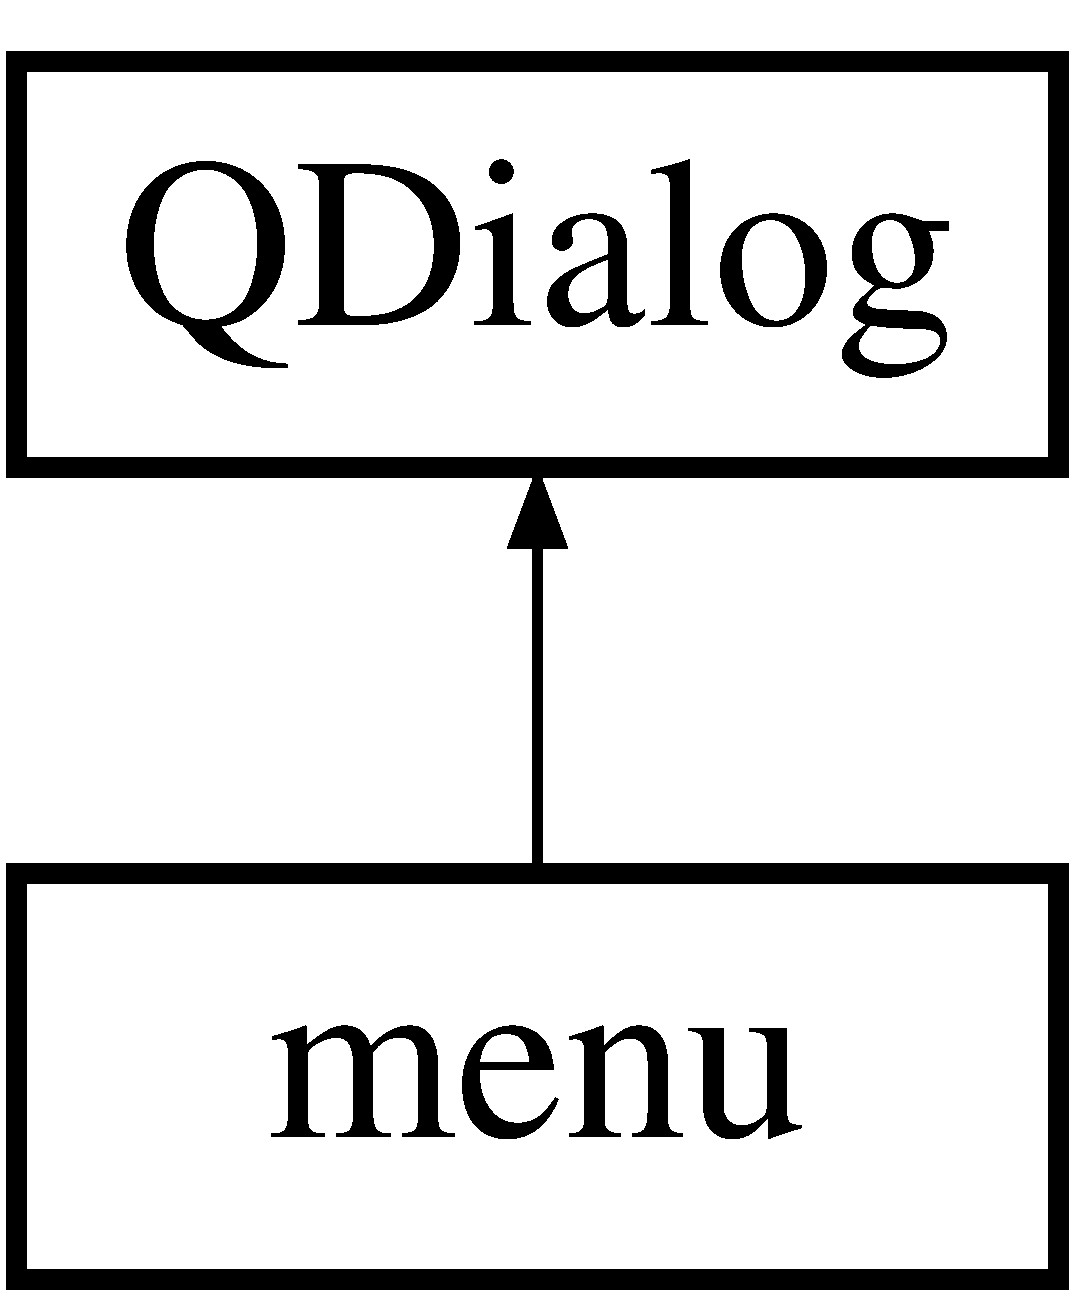
\includegraphics[height=2.000000cm]{classmenu}
\end{center}
\end{figure}
\subsection*{Public Slots}
\begin{DoxyCompactItemize}
\item 
void \hyperlink{classmenu_a4b63e5a7f04e55d65315f93980ba8a43}{on\+\_\+\+Registrar\+Paciente\+\_\+clicked} ()
\begin{DoxyCompactList}\small\item\em \hyperlink{classmenu_a4b63e5a7f04e55d65315f93980ba8a43}{menu\+::on\+\_\+\+Registrar\+Paciente\+\_\+clicked} \end{DoxyCompactList}\item 
void \hyperlink{classmenu_a62c11c56b58c852df09f28e2d47c82f6}{on\+\_\+ingresar\+Paciente\+\_\+clicked} ()
\begin{DoxyCompactList}\small\item\em \hyperlink{classmenu_a62c11c56b58c852df09f28e2d47c82f6}{menu\+::on\+\_\+ingresar\+Paciente\+\_\+clicked} \end{DoxyCompactList}\end{DoxyCompactItemize}
\subsection*{Public Member Functions}
\begin{DoxyCompactItemize}
\item 
\hyperlink{classmenu_aff7946ea9349eacaede63417ecea19cc}{menu} (Q\+Widget $\ast$parent=0)
\begin{DoxyCompactList}\small\item\em \hyperlink{classmenu_aff7946ea9349eacaede63417ecea19cc}{menu\+::menu} Es la función del constructor que controla lo que pasa al abrirse la ventana. \end{DoxyCompactList}\item 
\hyperlink{classmenu_a5efbd22f23289b42ed68d2a9bb431f35}{$\sim$menu} ()
\begin{DoxyCompactList}\small\item\em \hyperlink{classmenu_a5efbd22f23289b42ed68d2a9bb431f35}{menu\+::$\sim$menu} Es la función del destructor que controla lo que pasa al cerrarse la ventana. \end{DoxyCompactList}\end{DoxyCompactItemize}


\subsection{Detailed Description}
Esta clase maneja la conexión con la ventana de diálogo que nos permite elegir entre ingresar un paciente para hacerle la prueba de agilidad o registrar uno nuevo. 

\subsection{Constructor \& Destructor Documentation}
\mbox{\Hypertarget{classmenu_aff7946ea9349eacaede63417ecea19cc}\label{classmenu_aff7946ea9349eacaede63417ecea19cc}} 
\index{menu@{menu}!menu@{menu}}
\index{menu@{menu}!menu@{menu}}
\subsubsection{\texorpdfstring{menu()}{menu()}}
{\footnotesize\ttfamily menu\+::menu (\begin{DoxyParamCaption}\item[{Q\+Widget $\ast$}]{parent = {\ttfamily 0} }\end{DoxyParamCaption})\hspace{0.3cm}{\ttfamily [explicit]}}



\hyperlink{classmenu_aff7946ea9349eacaede63417ecea19cc}{menu\+::menu} Es la función del constructor que controla lo que pasa al abrirse la ventana. 

EL constructor de la clase.


\begin{DoxyParams}{Parameters}
{\em parent} & Es un puntero tipo Q\+Widget. \\
\hline
\end{DoxyParams}
\mbox{\Hypertarget{classmenu_a5efbd22f23289b42ed68d2a9bb431f35}\label{classmenu_a5efbd22f23289b42ed68d2a9bb431f35}} 
\index{menu@{menu}!````~menu@{$\sim$menu}}
\index{````~menu@{$\sim$menu}!menu@{menu}}
\subsubsection{\texorpdfstring{$\sim$menu()}{~menu()}}
{\footnotesize\ttfamily menu\+::$\sim$menu (\begin{DoxyParamCaption}{ }\end{DoxyParamCaption})}



\hyperlink{classmenu_a5efbd22f23289b42ed68d2a9bb431f35}{menu\+::$\sim$menu} Es la función del destructor que controla lo que pasa al cerrarse la ventana. 

EL destructor de la clase. 

\subsection{Member Function Documentation}
\mbox{\Hypertarget{classmenu_a62c11c56b58c852df09f28e2d47c82f6}\label{classmenu_a62c11c56b58c852df09f28e2d47c82f6}} 
\index{menu@{menu}!on\+\_\+ingresar\+Paciente\+\_\+clicked@{on\+\_\+ingresar\+Paciente\+\_\+clicked}}
\index{on\+\_\+ingresar\+Paciente\+\_\+clicked@{on\+\_\+ingresar\+Paciente\+\_\+clicked}!menu@{menu}}
\subsubsection{\texorpdfstring{on\+\_\+ingresar\+Paciente\+\_\+clicked}{on\_ingresarPaciente\_clicked}}
{\footnotesize\ttfamily void menu\+::on\+\_\+ingresar\+Paciente\+\_\+clicked (\begin{DoxyParamCaption}{ }\end{DoxyParamCaption})\hspace{0.3cm}{\ttfamily [slot]}}



\hyperlink{classmenu_a62c11c56b58c852df09f28e2d47c82f6}{menu\+::on\+\_\+ingresar\+Paciente\+\_\+clicked} 

Esta función es una slot privada que abre la ventana de verificación de paciente al hacer click en el botón ingresar\+Paciente. \mbox{\Hypertarget{classmenu_a4b63e5a7f04e55d65315f93980ba8a43}\label{classmenu_a4b63e5a7f04e55d65315f93980ba8a43}} 
\index{menu@{menu}!on\+\_\+\+Registrar\+Paciente\+\_\+clicked@{on\+\_\+\+Registrar\+Paciente\+\_\+clicked}}
\index{on\+\_\+\+Registrar\+Paciente\+\_\+clicked@{on\+\_\+\+Registrar\+Paciente\+\_\+clicked}!menu@{menu}}
\subsubsection{\texorpdfstring{on\+\_\+\+Registrar\+Paciente\+\_\+clicked}{on\_RegistrarPaciente\_clicked}}
{\footnotesize\ttfamily void menu\+::on\+\_\+\+Registrar\+Paciente\+\_\+clicked (\begin{DoxyParamCaption}{ }\end{DoxyParamCaption})\hspace{0.3cm}{\ttfamily [slot]}}



\hyperlink{classmenu_a4b63e5a7f04e55d65315f93980ba8a43}{menu\+::on\+\_\+\+Registrar\+Paciente\+\_\+clicked} 

Esta función es una slot privada que cierra la ventana al hacer click en el botón Registrar\+Paciente y nos direcciona a la ventana de registrar paciente. 

The documentation for this class was generated from the following files\+:\begin{DoxyCompactItemize}
\item 
/home/alseuser/\+Proecto\+\_\+final\+\_\+alse/\+P\+A/menu.\+h\item 
/home/alseuser/\+Proecto\+\_\+final\+\_\+alse/\+P\+A/menu.\+cpp\end{DoxyCompactItemize}

\hypertarget{classpaciente}{}\section{paciente Class Reference}
\label{classpaciente}\index{paciente@{paciente}}


Esta clase maneja la verificación de un paciente en la base de datos.  




{\ttfamily \#include $<$paciente.\+h$>$}

Inheritance diagram for paciente\+:\begin{figure}[H]
\begin{center}
\leavevmode
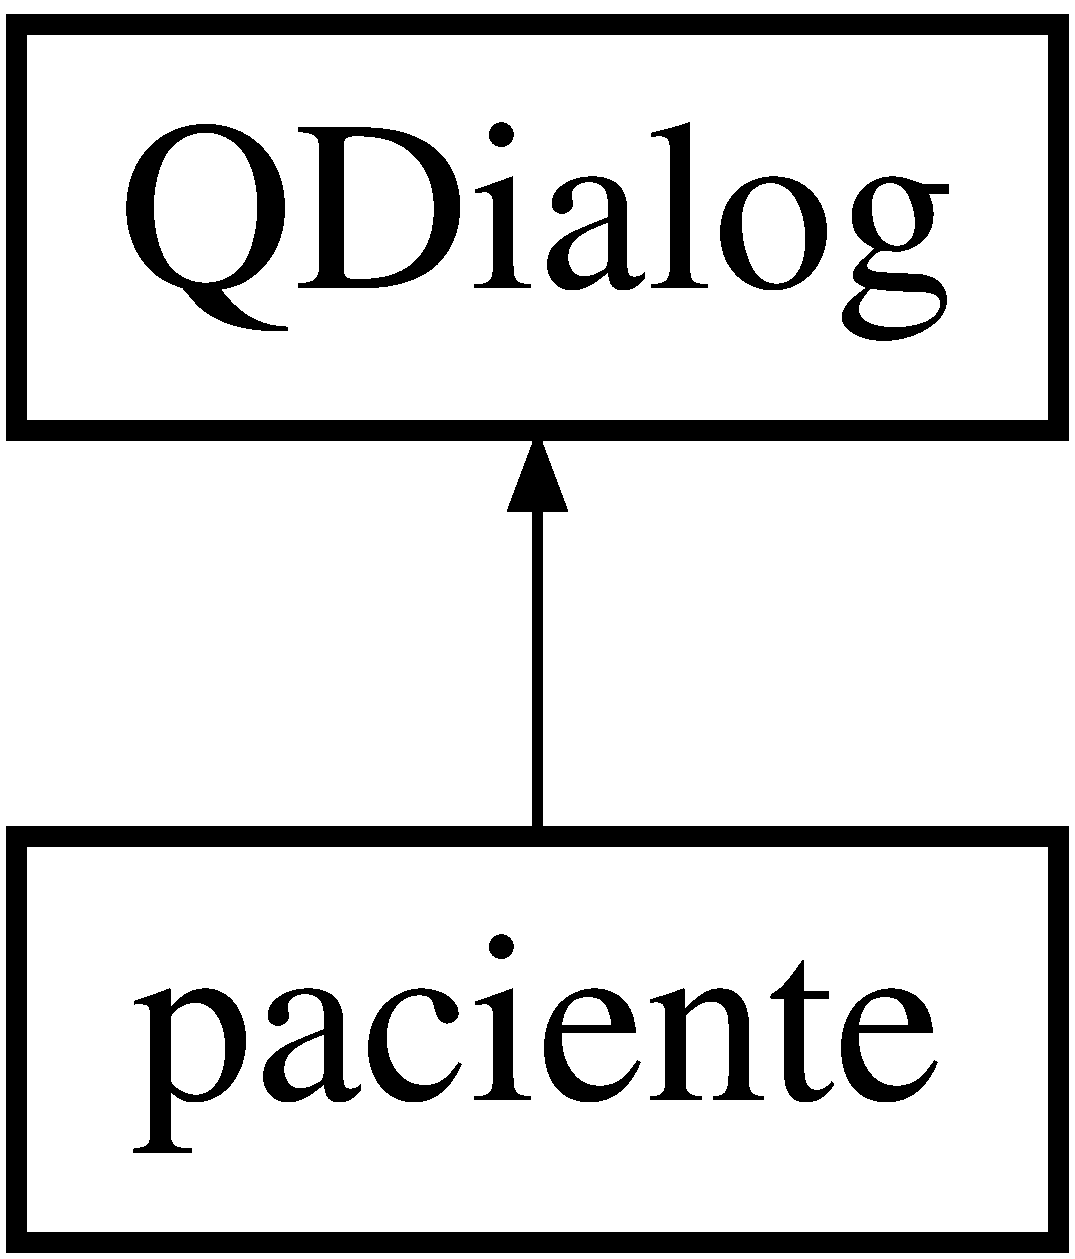
\includegraphics[height=2.000000cm]{classpaciente}
\end{center}
\end{figure}
\subsection*{Public Slots}
\begin{DoxyCompactItemize}
\item 
void \hyperlink{classpaciente_a6d34393d2eb8c21d66135346651a4995}{on\+\_\+\+Realizar\+Prueba\+\_\+clicked} ()
\begin{DoxyCompactList}\small\item\em \hyperlink{classpaciente_a6d34393d2eb8c21d66135346651a4995}{paciente\+::on\+\_\+\+Realizar\+Prueba\+\_\+clicked} \end{DoxyCompactList}\end{DoxyCompactItemize}
\subsection*{Public Member Functions}
\begin{DoxyCompactItemize}
\item 
\hyperlink{classpaciente_ad0ccef0b1f9db88970e6c748988cdf68}{paciente} (Q\+Widget $\ast$parent=0)
\begin{DoxyCompactList}\small\item\em \hyperlink{classpaciente_ad0ccef0b1f9db88970e6c748988cdf68}{paciente\+::paciente} Es la función del constructor que controla lo que pasa al abrirse la ventana. \end{DoxyCompactList}\item 
\hyperlink{classpaciente_aa2c0443ac761e3c01437ec3b051b1e5a}{$\sim$paciente} ()
\begin{DoxyCompactList}\small\item\em \hyperlink{classpaciente_aa2c0443ac761e3c01437ec3b051b1e5a}{paciente\+::$\sim$paciente} Es la función del destructor que controla lo que pasa al cerrarse la ventana. \end{DoxyCompactList}\item 
string \hyperlink{classpaciente_ade5b611666a067d54d8cee91bf737f2a}{get\+Nombre} () const
\begin{DoxyCompactList}\small\item\em \hyperlink{classpaciente_ade5b611666a067d54d8cee91bf737f2a}{paciente\+::get\+Nombre} \end{DoxyCompactList}\item 
void \hyperlink{classpaciente_aa1c002ee279da1512c06a30ab6f36cf8}{set\+Nombre} (const string \&value)
\begin{DoxyCompactList}\small\item\em \hyperlink{classpaciente_aa1c002ee279da1512c06a30ab6f36cf8}{paciente\+::set\+Nombre} \end{DoxyCompactList}\item 
string \hyperlink{classpaciente_a35eb76c2a62bf5942a81f3ab0dfa7ae6}{get\+Doci} () const
\begin{DoxyCompactList}\small\item\em \hyperlink{classpaciente_a35eb76c2a62bf5942a81f3ab0dfa7ae6}{paciente\+::get\+Doci} \end{DoxyCompactList}\item 
void \hyperlink{classpaciente_a98b1eb1d2344fde9ea082722eecd980a}{set\+Doci} (const string \&value)
\begin{DoxyCompactList}\small\item\em \hyperlink{classpaciente_a98b1eb1d2344fde9ea082722eecd980a}{paciente\+::set\+Doci} \end{DoxyCompactList}\end{DoxyCompactItemize}


\subsection{Detailed Description}
Esta clase maneja la verificación de un paciente en la base de datos. 

\subsection{Constructor \& Destructor Documentation}
\mbox{\Hypertarget{classpaciente_ad0ccef0b1f9db88970e6c748988cdf68}\label{classpaciente_ad0ccef0b1f9db88970e6c748988cdf68}} 
\index{paciente@{paciente}!paciente@{paciente}}
\index{paciente@{paciente}!paciente@{paciente}}
\subsubsection{\texorpdfstring{paciente()}{paciente()}}
{\footnotesize\ttfamily paciente\+::paciente (\begin{DoxyParamCaption}\item[{Q\+Widget $\ast$}]{parent = {\ttfamily 0} }\end{DoxyParamCaption})\hspace{0.3cm}{\ttfamily [explicit]}}



\hyperlink{classpaciente_ad0ccef0b1f9db88970e6c748988cdf68}{paciente\+::paciente} Es la función del constructor que controla lo que pasa al abrirse la ventana. 

EL constructor de la clase.


\begin{DoxyParams}{Parameters}
{\em parent} & \\
\hline
\end{DoxyParams}
\mbox{\Hypertarget{classpaciente_aa2c0443ac761e3c01437ec3b051b1e5a}\label{classpaciente_aa2c0443ac761e3c01437ec3b051b1e5a}} 
\index{paciente@{paciente}!````~paciente@{$\sim$paciente}}
\index{````~paciente@{$\sim$paciente}!paciente@{paciente}}
\subsubsection{\texorpdfstring{$\sim$paciente()}{~paciente()}}
{\footnotesize\ttfamily paciente\+::$\sim$paciente (\begin{DoxyParamCaption}{ }\end{DoxyParamCaption})}



\hyperlink{classpaciente_aa2c0443ac761e3c01437ec3b051b1e5a}{paciente\+::$\sim$paciente} Es la función del destructor que controla lo que pasa al cerrarse la ventana. 

EL destructor de la clase. 

\subsection{Member Function Documentation}
\mbox{\Hypertarget{classpaciente_a35eb76c2a62bf5942a81f3ab0dfa7ae6}\label{classpaciente_a35eb76c2a62bf5942a81f3ab0dfa7ae6}} 
\index{paciente@{paciente}!get\+Doci@{get\+Doci}}
\index{get\+Doci@{get\+Doci}!paciente@{paciente}}
\subsubsection{\texorpdfstring{get\+Doci()}{getDoci()}}
{\footnotesize\ttfamily string paciente\+::get\+Doci (\begin{DoxyParamCaption}{ }\end{DoxyParamCaption}) const}



\hyperlink{classpaciente_a35eb76c2a62bf5942a81f3ab0dfa7ae6}{paciente\+::get\+Doci} 

Es la función get de la variable \char`\"{}doci\char`\"{} que recupera o consigue el valor asignado en la función set para ser utilizado después. \begin{DoxyReturn}{Returns}
El valor ingresado en la función set. 
\end{DoxyReturn}
\mbox{\Hypertarget{classpaciente_ade5b611666a067d54d8cee91bf737f2a}\label{classpaciente_ade5b611666a067d54d8cee91bf737f2a}} 
\index{paciente@{paciente}!get\+Nombre@{get\+Nombre}}
\index{get\+Nombre@{get\+Nombre}!paciente@{paciente}}
\subsubsection{\texorpdfstring{get\+Nombre()}{getNombre()}}
{\footnotesize\ttfamily string paciente\+::get\+Nombre (\begin{DoxyParamCaption}{ }\end{DoxyParamCaption}) const}



\hyperlink{classpaciente_ade5b611666a067d54d8cee91bf737f2a}{paciente\+::get\+Nombre} 

Es la función get de la variable \char`\"{}nombre\char`\"{} que recupera o consigue el valor asignado en la función set para ser utilizado después. \begin{DoxyReturn}{Returns}
El valor ingresado en la función set. 
\end{DoxyReturn}
\mbox{\Hypertarget{classpaciente_a6d34393d2eb8c21d66135346651a4995}\label{classpaciente_a6d34393d2eb8c21d66135346651a4995}} 
\index{paciente@{paciente}!on\+\_\+\+Realizar\+Prueba\+\_\+clicked@{on\+\_\+\+Realizar\+Prueba\+\_\+clicked}}
\index{on\+\_\+\+Realizar\+Prueba\+\_\+clicked@{on\+\_\+\+Realizar\+Prueba\+\_\+clicked}!paciente@{paciente}}
\subsubsection{\texorpdfstring{on\+\_\+\+Realizar\+Prueba\+\_\+clicked}{on\_RealizarPrueba\_clicked}}
{\footnotesize\ttfamily void paciente\+::on\+\_\+\+Realizar\+Prueba\+\_\+clicked (\begin{DoxyParamCaption}{ }\end{DoxyParamCaption})\hspace{0.3cm}{\ttfamily [slot]}}



\hyperlink{classpaciente_a6d34393d2eb8c21d66135346651a4995}{paciente\+::on\+\_\+\+Realizar\+Prueba\+\_\+clicked} 

En esta función se asignan los datos ingresados en la ventana Q\+Dialog a unas variables con las que se verifica si los valores ingresados estan en la en la base de datos y si es así, se abre la ventana siguiente . \mbox{\Hypertarget{classpaciente_a98b1eb1d2344fde9ea082722eecd980a}\label{classpaciente_a98b1eb1d2344fde9ea082722eecd980a}} 
\index{paciente@{paciente}!set\+Doci@{set\+Doci}}
\index{set\+Doci@{set\+Doci}!paciente@{paciente}}
\subsubsection{\texorpdfstring{set\+Doci()}{setDoci()}}
{\footnotesize\ttfamily void paciente\+::set\+Doci (\begin{DoxyParamCaption}\item[{const string \&}]{value }\end{DoxyParamCaption})}



\hyperlink{classpaciente_a98b1eb1d2344fde9ea082722eecd980a}{paciente\+::set\+Doci} 

Es la función set de la variable \char`\"{}doci\char`\"{} que nos permite darle un valor a esta. 
\begin{DoxyParams}{Parameters}
{\em value} & Es un puntero tipo const string. \\
\hline
\end{DoxyParams}
\mbox{\Hypertarget{classpaciente_aa1c002ee279da1512c06a30ab6f36cf8}\label{classpaciente_aa1c002ee279da1512c06a30ab6f36cf8}} 
\index{paciente@{paciente}!set\+Nombre@{set\+Nombre}}
\index{set\+Nombre@{set\+Nombre}!paciente@{paciente}}
\subsubsection{\texorpdfstring{set\+Nombre()}{setNombre()}}
{\footnotesize\ttfamily void paciente\+::set\+Nombre (\begin{DoxyParamCaption}\item[{const string \&}]{value }\end{DoxyParamCaption})}



\hyperlink{classpaciente_aa1c002ee279da1512c06a30ab6f36cf8}{paciente\+::set\+Nombre} 

Es la función set de la variable \char`\"{}nombre\char`\"{} que nos permite darle un valor a esta. 
\begin{DoxyParams}{Parameters}
{\em value} & Es un puntero tipo const string. \\
\hline
\end{DoxyParams}


The documentation for this class was generated from the following files\+:\begin{DoxyCompactItemize}
\item 
/home/alseuser/\+Proecto\+\_\+final\+\_\+alse/\+P\+A/paciente.\+h\item 
/home/alseuser/\+Proecto\+\_\+final\+\_\+alse/\+P\+A/paciente.\+cpp\end{DoxyCompactItemize}

\hypertarget{classprueba}{}\section{prueba Class Reference}
\label{classprueba}\index{prueba@{prueba}}


Esta clase maneja la ventana de la prueba de agilidad para el paciente.  




{\ttfamily \#include $<$prueba.\+h$>$}

Inheritance diagram for prueba\+:\begin{figure}[H]
\begin{center}
\leavevmode
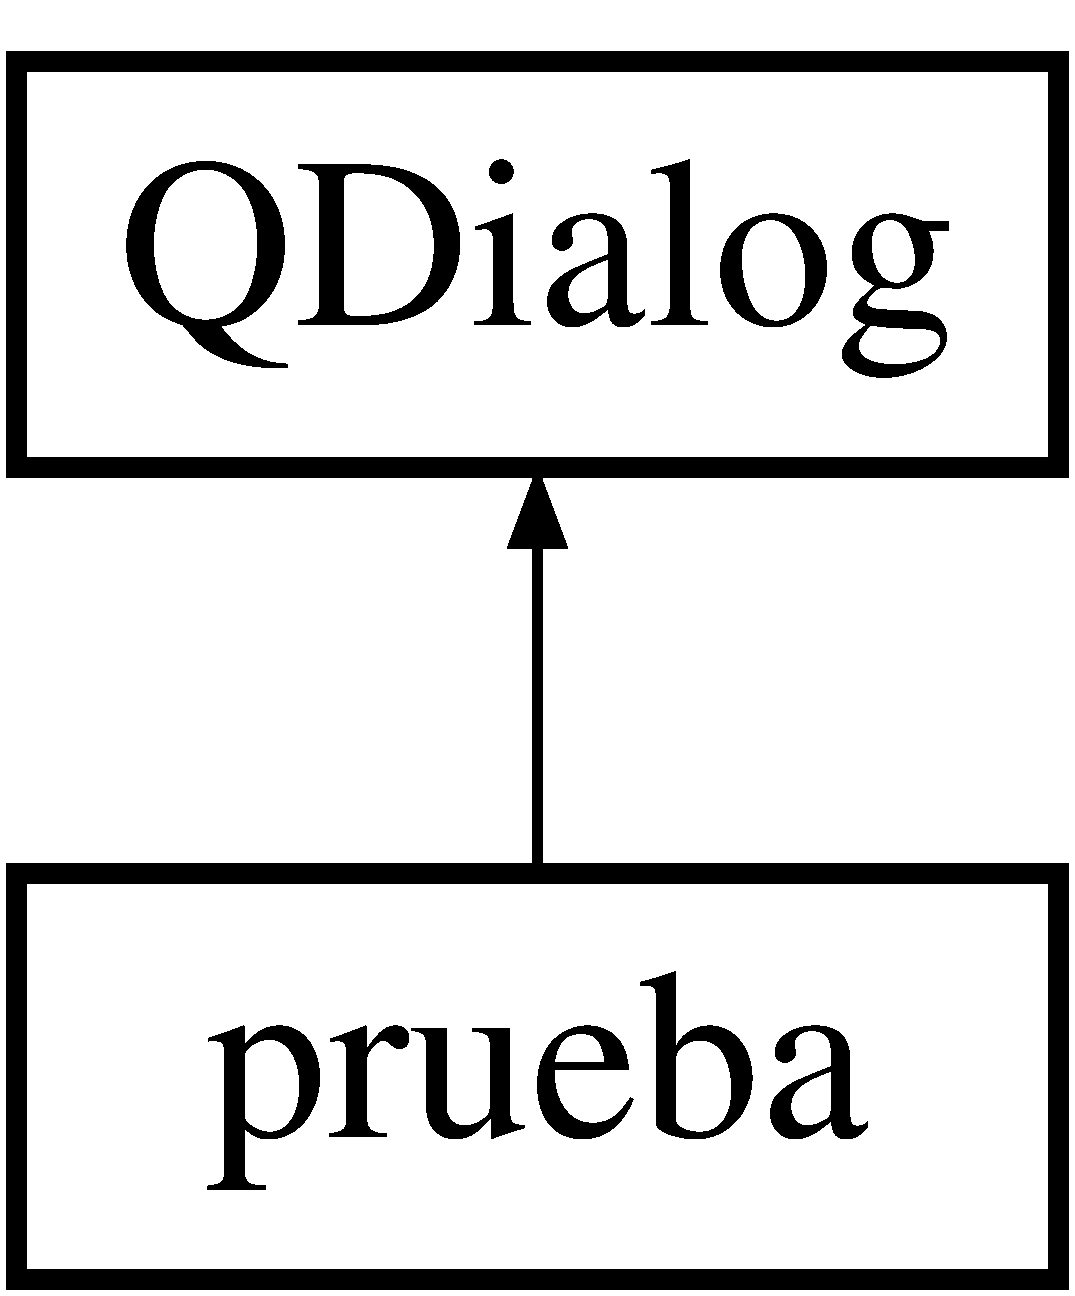
\includegraphics[height=2.000000cm]{classprueba}
\end{center}
\end{figure}
\subsection*{Public Slots}
\begin{DoxyCompactItemize}
\item 
\mbox{\Hypertarget{classprueba_a149805ab01c4101c9f183029a3621a10}\label{classprueba_a149805ab01c4101c9f183029a3621a10}} 
void \hyperlink{classprueba_a149805ab01c4101c9f183029a3621a10}{cambio\+\_\+estado} (void)
\begin{DoxyCompactList}\small\item\em \hyperlink{classprueba_a149805ab01c4101c9f183029a3621a10}{prueba\+::cambio\+\_\+estado} Esta función nos permite hacer que los leds se enciendan al cambiar los estados de manera aleatoria. \end{DoxyCompactList}\item 
void \hyperlink{classprueba_a09d5326f33ef9cfafd86237e733c1093}{on\+\_\+boton1\+\_\+clicked} ()
\begin{DoxyCompactList}\small\item\em \hyperlink{classprueba_a09d5326f33ef9cfafd86237e733c1093}{prueba\+::on\+\_\+boton1\+\_\+clicked} \end{DoxyCompactList}\item 
void \hyperlink{classprueba_ae81b6c5c5782c2348f88bdb0f34b163f}{on\+\_\+boton2\+\_\+clicked} ()
\begin{DoxyCompactList}\small\item\em \hyperlink{classprueba_ae81b6c5c5782c2348f88bdb0f34b163f}{prueba\+::on\+\_\+boton2\+\_\+clicked} \end{DoxyCompactList}\item 
void \hyperlink{classprueba_a622258b2f43536c572613dc4bc3e4e65}{on\+\_\+boton3\+\_\+clicked} ()
\begin{DoxyCompactList}\small\item\em \hyperlink{classprueba_a622258b2f43536c572613dc4bc3e4e65}{prueba\+::on\+\_\+boton3\+\_\+clicked} \end{DoxyCompactList}\item 
void \hyperlink{classprueba_a3de0793fdcb9d6c63382a665ba435736}{on\+\_\+boton4\+\_\+clicked} ()
\begin{DoxyCompactList}\small\item\em \hyperlink{classprueba_a3de0793fdcb9d6c63382a665ba435736}{prueba\+::on\+\_\+boton4\+\_\+clicked} \end{DoxyCompactList}\item 
void \hyperlink{classprueba_a5fe7941d4155bd83e2746e6d29aa9bdb}{on\+\_\+boton5\+\_\+clicked} ()
\begin{DoxyCompactList}\small\item\em \hyperlink{classprueba_a5fe7941d4155bd83e2746e6d29aa9bdb}{prueba\+::on\+\_\+boton5\+\_\+clicked} \end{DoxyCompactList}\item 
void \hyperlink{classprueba_a8d324e5b5d7e37fd16e9e287bbcb5ea5}{on\+\_\+boton6\+\_\+clicked} ()
\begin{DoxyCompactList}\small\item\em \hyperlink{classprueba_a8d324e5b5d7e37fd16e9e287bbcb5ea5}{prueba\+::on\+\_\+boton6\+\_\+clicked} \end{DoxyCompactList}\item 
void \hyperlink{classprueba_a22855fb3346928da988d6a8ed4dd466b}{on\+\_\+boton7\+\_\+clicked} ()
\begin{DoxyCompactList}\small\item\em \hyperlink{classprueba_a22855fb3346928da988d6a8ed4dd466b}{prueba\+::on\+\_\+boton7\+\_\+clicked} \end{DoxyCompactList}\item 
void \hyperlink{classprueba_adead6ef4b051b587a91e3fd1037a65dd}{on\+\_\+boton8\+\_\+clicked} ()
\begin{DoxyCompactList}\small\item\em \hyperlink{classprueba_adead6ef4b051b587a91e3fd1037a65dd}{prueba\+::on\+\_\+boton8\+\_\+clicked} \end{DoxyCompactList}\item 
void \hyperlink{classprueba_afb0931a028ade1ee29a8dda28acf1506}{on\+\_\+boton9\+\_\+clicked} ()
\begin{DoxyCompactList}\small\item\em \hyperlink{classprueba_afb0931a028ade1ee29a8dda28acf1506}{prueba\+::on\+\_\+boton9\+\_\+clicked} \end{DoxyCompactList}\item 
void \hyperlink{classprueba_a514abf87fbde22efc7ea3cba147e733c}{on\+\_\+boton10\+\_\+clicked} ()
\begin{DoxyCompactList}\small\item\em \hyperlink{classprueba_a514abf87fbde22efc7ea3cba147e733c}{prueba\+::on\+\_\+boton10\+\_\+clicked} \end{DoxyCompactList}\item 
void \hyperlink{classprueba_a332ffe63208038c15521b078581fbd24}{on\+\_\+boton11\+\_\+clicked} ()
\begin{DoxyCompactList}\small\item\em \hyperlink{classprueba_a332ffe63208038c15521b078581fbd24}{prueba\+::on\+\_\+boton11\+\_\+clicked} \end{DoxyCompactList}\end{DoxyCompactItemize}
\subsection*{Public Member Functions}
\begin{DoxyCompactItemize}
\item 
\hyperlink{classprueba_a24f54c7bdd250ae7c191204b6640e76a}{prueba} (Q\+Widget $\ast$parent=0)
\begin{DoxyCompactList}\small\item\em \hyperlink{classprueba_a24f54c7bdd250ae7c191204b6640e76a}{prueba\+::prueba} Es la función del constructor que controla lo que pasa al abrirse la ventana. \end{DoxyCompactList}\item 
\hyperlink{classprueba_a10ec83347646102027f40a34f8cc9688}{$\sim$prueba} ()
\begin{DoxyCompactList}\small\item\em \hyperlink{classprueba_a10ec83347646102027f40a34f8cc9688}{prueba\+::$\sim$prueba} Es la función del destructor que controla lo que pasa al cerrarse la ventana. \end{DoxyCompactList}\item 
void \hyperlink{classprueba_ac7bf490420a1bd8080157ce2e2d6b78c}{insertar} ()
\begin{DoxyCompactList}\small\item\em \hyperlink{classprueba_ac7bf490420a1bd8080157ce2e2d6b78c}{prueba\+::insertar} \end{DoxyCompactList}\item 
void \hyperlink{classprueba_ad26285fa9b7055591708f9a31223353b}{resultados} ()
\begin{DoxyCompactList}\small\item\em \hyperlink{classprueba_ad26285fa9b7055591708f9a31223353b}{prueba\+::resultados} \end{DoxyCompactList}\end{DoxyCompactItemize}


\subsection{Detailed Description}
Esta clase maneja la ventana de la prueba de agilidad para el paciente. 

\subsection{Constructor \& Destructor Documentation}
\mbox{\Hypertarget{classprueba_a24f54c7bdd250ae7c191204b6640e76a}\label{classprueba_a24f54c7bdd250ae7c191204b6640e76a}} 
\index{prueba@{prueba}!prueba@{prueba}}
\index{prueba@{prueba}!prueba@{prueba}}
\subsubsection{\texorpdfstring{prueba()}{prueba()}}
{\footnotesize\ttfamily prueba\+::prueba (\begin{DoxyParamCaption}\item[{Q\+Widget $\ast$}]{parent = {\ttfamily 0} }\end{DoxyParamCaption})\hspace{0.3cm}{\ttfamily [explicit]}}



\hyperlink{classprueba_a24f54c7bdd250ae7c191204b6640e76a}{prueba\+::prueba} Es la función del constructor que controla lo que pasa al abrirse la ventana. 

EL constructor de la clase.


\begin{DoxyParams}{Parameters}
{\em parent} & Es un puntero tipo Q\+Widget. \\
\hline
\end{DoxyParams}
\mbox{\Hypertarget{classprueba_a10ec83347646102027f40a34f8cc9688}\label{classprueba_a10ec83347646102027f40a34f8cc9688}} 
\index{prueba@{prueba}!````~prueba@{$\sim$prueba}}
\index{````~prueba@{$\sim$prueba}!prueba@{prueba}}
\subsubsection{\texorpdfstring{$\sim$prueba()}{~prueba()}}
{\footnotesize\ttfamily prueba\+::$\sim$prueba (\begin{DoxyParamCaption}{ }\end{DoxyParamCaption})}



\hyperlink{classprueba_a10ec83347646102027f40a34f8cc9688}{prueba\+::$\sim$prueba} Es la función del destructor que controla lo que pasa al cerrarse la ventana. 

EL destructor de la clase. 

\subsection{Member Function Documentation}
\mbox{\Hypertarget{classprueba_ac7bf490420a1bd8080157ce2e2d6b78c}\label{classprueba_ac7bf490420a1bd8080157ce2e2d6b78c}} 
\index{prueba@{prueba}!insertar@{insertar}}
\index{insertar@{insertar}!prueba@{prueba}}
\subsubsection{\texorpdfstring{insertar()}{insertar()}}
{\footnotesize\ttfamily void prueba\+::insertar (\begin{DoxyParamCaption}{ }\end{DoxyParamCaption})}



\hyperlink{classprueba_ac7bf490420a1bd8080157ce2e2d6b78c}{prueba\+::insertar} 

Esta función sirve para insertar los datos obtenidos en la prueba en la base de datos. \mbox{\Hypertarget{classprueba_a514abf87fbde22efc7ea3cba147e733c}\label{classprueba_a514abf87fbde22efc7ea3cba147e733c}} 
\index{prueba@{prueba}!on\+\_\+boton10\+\_\+clicked@{on\+\_\+boton10\+\_\+clicked}}
\index{on\+\_\+boton10\+\_\+clicked@{on\+\_\+boton10\+\_\+clicked}!prueba@{prueba}}
\subsubsection{\texorpdfstring{on\+\_\+boton10\+\_\+clicked}{on\_boton10\_clicked}}
{\footnotesize\ttfamily void prueba\+::on\+\_\+boton10\+\_\+clicked (\begin{DoxyParamCaption}{ }\end{DoxyParamCaption})\hspace{0.3cm}{\ttfamily [slot]}}



\hyperlink{classprueba_a514abf87fbde22efc7ea3cba147e733c}{prueba\+::on\+\_\+boton10\+\_\+clicked} 

Esta función nos permite comparar si el botón que está pulsando el paciente es igual al botón que está prendido y en caso de ser así aumenta el contador de los aciertos, al hacer click en el boton 10. \mbox{\Hypertarget{classprueba_a332ffe63208038c15521b078581fbd24}\label{classprueba_a332ffe63208038c15521b078581fbd24}} 
\index{prueba@{prueba}!on\+\_\+boton11\+\_\+clicked@{on\+\_\+boton11\+\_\+clicked}}
\index{on\+\_\+boton11\+\_\+clicked@{on\+\_\+boton11\+\_\+clicked}!prueba@{prueba}}
\subsubsection{\texorpdfstring{on\+\_\+boton11\+\_\+clicked}{on\_boton11\_clicked}}
{\footnotesize\ttfamily void prueba\+::on\+\_\+boton11\+\_\+clicked (\begin{DoxyParamCaption}{ }\end{DoxyParamCaption})\hspace{0.3cm}{\ttfamily [slot]}}



\hyperlink{classprueba_a332ffe63208038c15521b078581fbd24}{prueba\+::on\+\_\+boton11\+\_\+clicked} 

Esta función nos permite comparar si el botón que está pulsando el paciente es igual al botón que está prendido y en caso de ser así aumenta el contador de los aciertos, al hacer click en el boton 11. \mbox{\Hypertarget{classprueba_a09d5326f33ef9cfafd86237e733c1093}\label{classprueba_a09d5326f33ef9cfafd86237e733c1093}} 
\index{prueba@{prueba}!on\+\_\+boton1\+\_\+clicked@{on\+\_\+boton1\+\_\+clicked}}
\index{on\+\_\+boton1\+\_\+clicked@{on\+\_\+boton1\+\_\+clicked}!prueba@{prueba}}
\subsubsection{\texorpdfstring{on\+\_\+boton1\+\_\+clicked}{on\_boton1\_clicked}}
{\footnotesize\ttfamily void prueba\+::on\+\_\+boton1\+\_\+clicked (\begin{DoxyParamCaption}{ }\end{DoxyParamCaption})\hspace{0.3cm}{\ttfamily [slot]}}



\hyperlink{classprueba_a09d5326f33ef9cfafd86237e733c1093}{prueba\+::on\+\_\+boton1\+\_\+clicked} 

Esta función nos permite comparar si el botón que está pulsando el paciente es igual al botón que está prendido y en caso de ser así aumenta el contador de los aciertos, al hacer click en el boton 1. \mbox{\Hypertarget{classprueba_ae81b6c5c5782c2348f88bdb0f34b163f}\label{classprueba_ae81b6c5c5782c2348f88bdb0f34b163f}} 
\index{prueba@{prueba}!on\+\_\+boton2\+\_\+clicked@{on\+\_\+boton2\+\_\+clicked}}
\index{on\+\_\+boton2\+\_\+clicked@{on\+\_\+boton2\+\_\+clicked}!prueba@{prueba}}
\subsubsection{\texorpdfstring{on\+\_\+boton2\+\_\+clicked}{on\_boton2\_clicked}}
{\footnotesize\ttfamily void prueba\+::on\+\_\+boton2\+\_\+clicked (\begin{DoxyParamCaption}{ }\end{DoxyParamCaption})\hspace{0.3cm}{\ttfamily [slot]}}



\hyperlink{classprueba_ae81b6c5c5782c2348f88bdb0f34b163f}{prueba\+::on\+\_\+boton2\+\_\+clicked} 

Esta función nos permite comparar si el botón que está pulsando el paciente es igual al botón que está prendido y en caso de ser así aumenta el contador de los aciertos, al hacer click en el boton 2. \mbox{\Hypertarget{classprueba_a622258b2f43536c572613dc4bc3e4e65}\label{classprueba_a622258b2f43536c572613dc4bc3e4e65}} 
\index{prueba@{prueba}!on\+\_\+boton3\+\_\+clicked@{on\+\_\+boton3\+\_\+clicked}}
\index{on\+\_\+boton3\+\_\+clicked@{on\+\_\+boton3\+\_\+clicked}!prueba@{prueba}}
\subsubsection{\texorpdfstring{on\+\_\+boton3\+\_\+clicked}{on\_boton3\_clicked}}
{\footnotesize\ttfamily void prueba\+::on\+\_\+boton3\+\_\+clicked (\begin{DoxyParamCaption}{ }\end{DoxyParamCaption})\hspace{0.3cm}{\ttfamily [slot]}}



\hyperlink{classprueba_a622258b2f43536c572613dc4bc3e4e65}{prueba\+::on\+\_\+boton3\+\_\+clicked} 

Esta función nos permite comparar si el botón que está pulsando el paciente es igual al botón que está prendido y en caso de ser así aumenta el contador de los aciertos, al hacer click en el boton 3. \mbox{\Hypertarget{classprueba_a3de0793fdcb9d6c63382a665ba435736}\label{classprueba_a3de0793fdcb9d6c63382a665ba435736}} 
\index{prueba@{prueba}!on\+\_\+boton4\+\_\+clicked@{on\+\_\+boton4\+\_\+clicked}}
\index{on\+\_\+boton4\+\_\+clicked@{on\+\_\+boton4\+\_\+clicked}!prueba@{prueba}}
\subsubsection{\texorpdfstring{on\+\_\+boton4\+\_\+clicked}{on\_boton4\_clicked}}
{\footnotesize\ttfamily void prueba\+::on\+\_\+boton4\+\_\+clicked (\begin{DoxyParamCaption}{ }\end{DoxyParamCaption})\hspace{0.3cm}{\ttfamily [slot]}}



\hyperlink{classprueba_a3de0793fdcb9d6c63382a665ba435736}{prueba\+::on\+\_\+boton4\+\_\+clicked} 

Esta función nos permite comparar si el botón que está pulsando el paciente es igual al botón que está prendido y en caso de ser así aumenta el contador de los aciertos, al hacer click en el boton 4. \mbox{\Hypertarget{classprueba_a5fe7941d4155bd83e2746e6d29aa9bdb}\label{classprueba_a5fe7941d4155bd83e2746e6d29aa9bdb}} 
\index{prueba@{prueba}!on\+\_\+boton5\+\_\+clicked@{on\+\_\+boton5\+\_\+clicked}}
\index{on\+\_\+boton5\+\_\+clicked@{on\+\_\+boton5\+\_\+clicked}!prueba@{prueba}}
\subsubsection{\texorpdfstring{on\+\_\+boton5\+\_\+clicked}{on\_boton5\_clicked}}
{\footnotesize\ttfamily void prueba\+::on\+\_\+boton5\+\_\+clicked (\begin{DoxyParamCaption}{ }\end{DoxyParamCaption})\hspace{0.3cm}{\ttfamily [slot]}}



\hyperlink{classprueba_a5fe7941d4155bd83e2746e6d29aa9bdb}{prueba\+::on\+\_\+boton5\+\_\+clicked} 

Esta función nos permite comparar si el botón que está pulsando el paciente es igual al botón que está prendido y en caso de ser así aumenta el contador de los aciertos, al hacer click en el boton 5. \mbox{\Hypertarget{classprueba_a8d324e5b5d7e37fd16e9e287bbcb5ea5}\label{classprueba_a8d324e5b5d7e37fd16e9e287bbcb5ea5}} 
\index{prueba@{prueba}!on\+\_\+boton6\+\_\+clicked@{on\+\_\+boton6\+\_\+clicked}}
\index{on\+\_\+boton6\+\_\+clicked@{on\+\_\+boton6\+\_\+clicked}!prueba@{prueba}}
\subsubsection{\texorpdfstring{on\+\_\+boton6\+\_\+clicked}{on\_boton6\_clicked}}
{\footnotesize\ttfamily void prueba\+::on\+\_\+boton6\+\_\+clicked (\begin{DoxyParamCaption}{ }\end{DoxyParamCaption})\hspace{0.3cm}{\ttfamily [slot]}}



\hyperlink{classprueba_a8d324e5b5d7e37fd16e9e287bbcb5ea5}{prueba\+::on\+\_\+boton6\+\_\+clicked} 

Esta función nos permite comparar si el botón que está pulsando el paciente es igual al botón que está prendido y en caso de ser así aumenta el contador de los aciertos, al hacer click en el boton 6. \mbox{\Hypertarget{classprueba_a22855fb3346928da988d6a8ed4dd466b}\label{classprueba_a22855fb3346928da988d6a8ed4dd466b}} 
\index{prueba@{prueba}!on\+\_\+boton7\+\_\+clicked@{on\+\_\+boton7\+\_\+clicked}}
\index{on\+\_\+boton7\+\_\+clicked@{on\+\_\+boton7\+\_\+clicked}!prueba@{prueba}}
\subsubsection{\texorpdfstring{on\+\_\+boton7\+\_\+clicked}{on\_boton7\_clicked}}
{\footnotesize\ttfamily void prueba\+::on\+\_\+boton7\+\_\+clicked (\begin{DoxyParamCaption}{ }\end{DoxyParamCaption})\hspace{0.3cm}{\ttfamily [slot]}}



\hyperlink{classprueba_a22855fb3346928da988d6a8ed4dd466b}{prueba\+::on\+\_\+boton7\+\_\+clicked} 

Esta función nos permite comparar si el botón que está pulsando el paciente es igual al botón que está prendido y en caso de ser así aumenta el contador de los aciertos, al hacer click en el boton 7. \mbox{\Hypertarget{classprueba_adead6ef4b051b587a91e3fd1037a65dd}\label{classprueba_adead6ef4b051b587a91e3fd1037a65dd}} 
\index{prueba@{prueba}!on\+\_\+boton8\+\_\+clicked@{on\+\_\+boton8\+\_\+clicked}}
\index{on\+\_\+boton8\+\_\+clicked@{on\+\_\+boton8\+\_\+clicked}!prueba@{prueba}}
\subsubsection{\texorpdfstring{on\+\_\+boton8\+\_\+clicked}{on\_boton8\_clicked}}
{\footnotesize\ttfamily void prueba\+::on\+\_\+boton8\+\_\+clicked (\begin{DoxyParamCaption}{ }\end{DoxyParamCaption})\hspace{0.3cm}{\ttfamily [slot]}}



\hyperlink{classprueba_adead6ef4b051b587a91e3fd1037a65dd}{prueba\+::on\+\_\+boton8\+\_\+clicked} 

Esta función nos permite comparar si el botón que está pulsando el paciente es igual al botón que está prendido y en caso de ser así aumenta el contador de los aciertos, al hacer click en el boton 8. \mbox{\Hypertarget{classprueba_afb0931a028ade1ee29a8dda28acf1506}\label{classprueba_afb0931a028ade1ee29a8dda28acf1506}} 
\index{prueba@{prueba}!on\+\_\+boton9\+\_\+clicked@{on\+\_\+boton9\+\_\+clicked}}
\index{on\+\_\+boton9\+\_\+clicked@{on\+\_\+boton9\+\_\+clicked}!prueba@{prueba}}
\subsubsection{\texorpdfstring{on\+\_\+boton9\+\_\+clicked}{on\_boton9\_clicked}}
{\footnotesize\ttfamily void prueba\+::on\+\_\+boton9\+\_\+clicked (\begin{DoxyParamCaption}{ }\end{DoxyParamCaption})\hspace{0.3cm}{\ttfamily [slot]}}



\hyperlink{classprueba_afb0931a028ade1ee29a8dda28acf1506}{prueba\+::on\+\_\+boton9\+\_\+clicked} 

Esta función nos permite comparar si el botón que está pulsando el paciente es igual al botón que está prendido y en caso de ser así aumenta el contador de los aciertos, al hacer click en el boton 9. \mbox{\Hypertarget{classprueba_ad26285fa9b7055591708f9a31223353b}\label{classprueba_ad26285fa9b7055591708f9a31223353b}} 
\index{prueba@{prueba}!resultados@{resultados}}
\index{resultados@{resultados}!prueba@{prueba}}
\subsubsection{\texorpdfstring{resultados()}{resultados()}}
{\footnotesize\ttfamily void prueba\+::resultados (\begin{DoxyParamCaption}{ }\end{DoxyParamCaption})}



\hyperlink{classprueba_ad26285fa9b7055591708f9a31223353b}{prueba\+::resultados} 

Esta función nos muestra los resultados obtenidos en la prueba como los aciertos y la nota. 

The documentation for this class was generated from the following files\+:\begin{DoxyCompactItemize}
\item 
/home/alseuser/\+Proecto\+\_\+final\+\_\+alse/\+P\+A/prueba.\+h\item 
/home/alseuser/\+Proecto\+\_\+final\+\_\+alse/\+P\+A/prueba.\+cpp\end{DoxyCompactItemize}

\hypertarget{classregpc}{}\section{regpc Class Reference}
\label{classregpc}\index{regpc@{regpc}}


Esta clase maneja la conexión con la ventana de dialogo Q\+Dialog donde se registran los datos de un paciente nuevo.  




{\ttfamily \#include $<$regpc.\+h$>$}

Inheritance diagram for regpc\+:\begin{figure}[H]
\begin{center}
\leavevmode
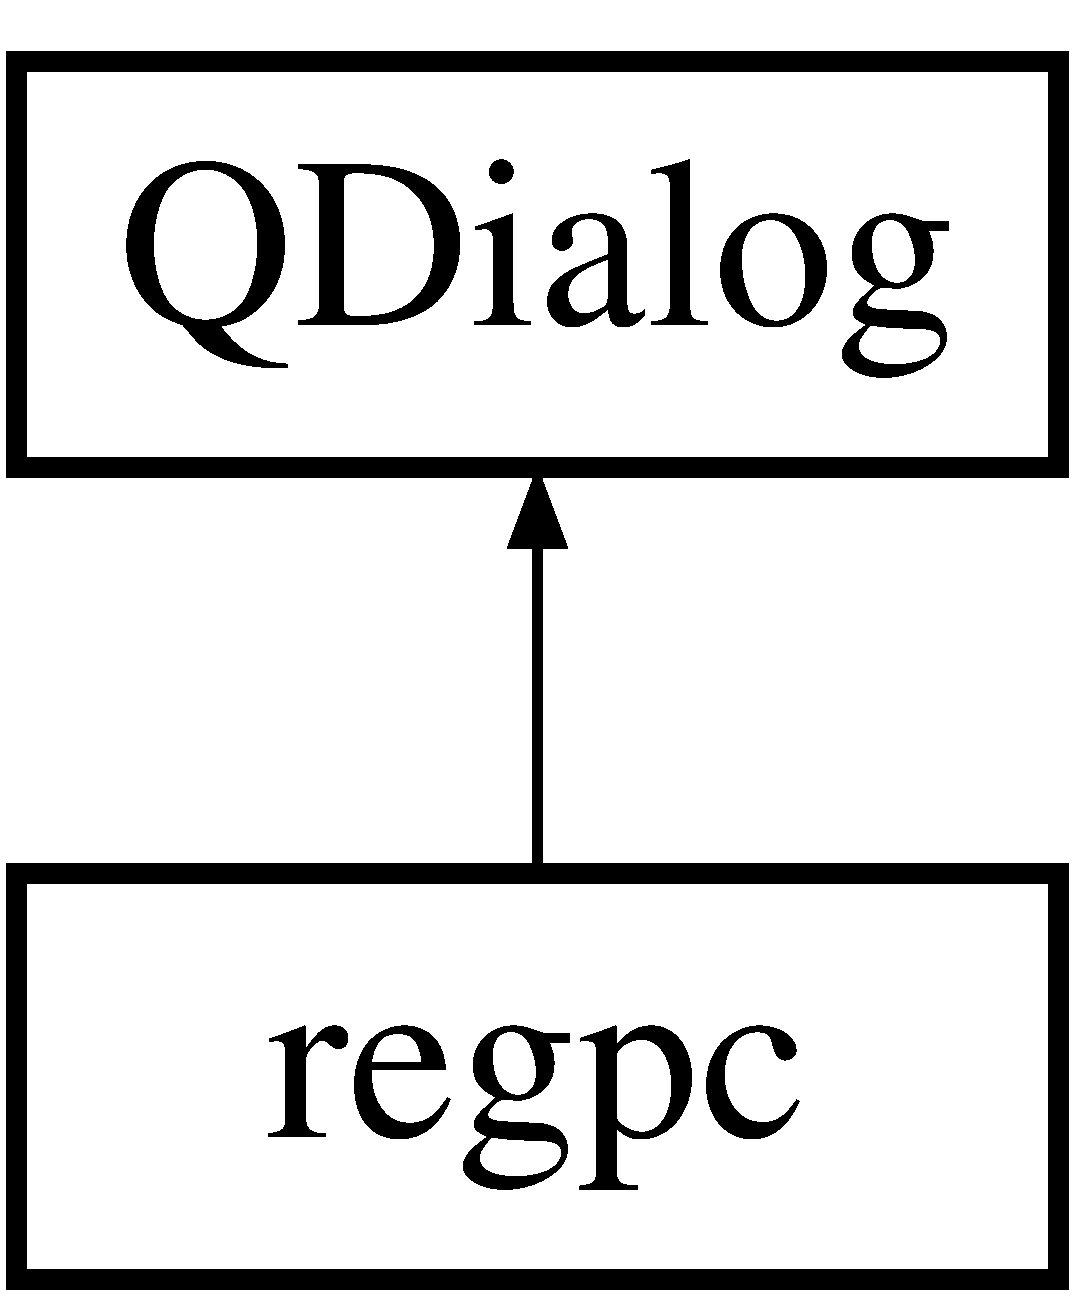
\includegraphics[height=2.000000cm]{classregpc}
\end{center}
\end{figure}
\subsection*{Public Slots}
\begin{DoxyCompactItemize}
\item 
void \hyperlink{classregpc_a0126d0e41901f442a138c3fc2236df9a}{on\+\_\+guardar\+\_\+clicked} ()
\begin{DoxyCompactList}\small\item\em \hyperlink{classregpc_a0126d0e41901f442a138c3fc2236df9a}{regpc\+::on\+\_\+guardar\+\_\+clicked} \end{DoxyCompactList}\item 
void \hyperlink{classregpc_aebdc318917c7ea9b3a2aca0e8155f854}{on\+\_\+generof\+\_\+clicked} ()
\begin{DoxyCompactList}\small\item\em \hyperlink{classregpc_aebdc318917c7ea9b3a2aca0e8155f854}{regpc\+::on\+\_\+generof\+\_\+clicked} \end{DoxyCompactList}\item 
void \hyperlink{classregpc_a5e7c8c456ee0a0a51e341d00bd0d8ba3}{on\+\_\+generom\+\_\+clicked} ()
\begin{DoxyCompactList}\small\item\em \hyperlink{classregpc_a5e7c8c456ee0a0a51e341d00bd0d8ba3}{regpc\+::on\+\_\+generom\+\_\+clicked} \end{DoxyCompactList}\end{DoxyCompactItemize}
\subsection*{Public Member Functions}
\begin{DoxyCompactItemize}
\item 
\hyperlink{classregpc_a0e746dd80042db7863f1acc0eceb3e0e}{regpc} (Q\+Widget $\ast$parent=0)
\begin{DoxyCompactList}\small\item\em \hyperlink{classregpc_a0e746dd80042db7863f1acc0eceb3e0e}{regpc\+::regpc} Es la función del constructor que controla lo que pasa al abrirse la ventana. \end{DoxyCompactList}\item 
\hyperlink{classregpc_a44345c70fea1c353bde3cd00e4a05c1d}{$\sim$regpc} ()
\begin{DoxyCompactList}\small\item\em \hyperlink{classregpc_a44345c70fea1c353bde3cd00e4a05c1d}{regpc\+::$\sim$regpc} Es la función del destructor que controla lo que pasa al cerrarse la ventana. \end{DoxyCompactList}\item 
void \hyperlink{classregpc_a4c2805dbeac86a39d8afd591c7f14ec9}{calcularedad} ()
\begin{DoxyCompactList}\small\item\em \hyperlink{classregpc_a4c2805dbeac86a39d8afd591c7f14ec9}{regpc\+::calcularedad} \end{DoxyCompactList}\end{DoxyCompactItemize}
\subsection*{Public Attributes}
\begin{DoxyCompactItemize}
\item 
string \hyperlink{classregpc_a95b954b79eb473167a8e631833d756ad}{nombre}
\item 
string \hyperlink{classregpc_a8b52a6da10996801ea903a96ae8123da}{apellido}
\item 
string \hyperlink{classregpc_a7b918d9a415903d63944d3ef17e48c3d}{docident}
\item 
string \hyperlink{classregpc_a0db133a320356ff6a456cee7f2d34720}{fn}
\item 
string \hyperlink{classregpc_a316ab55a02639999cc96f751997a521e}{direccion}
\item 
string \hyperlink{classregpc_ad7cee8fe68a32c50e6de8c621e3c61bc}{gn}
\item 
string \hyperlink{classregpc_a76fa61f1dbcfb75c08707c4c9cb71b43}{rz}
\item 
string \hyperlink{classregpc_a3634b2c40b40e029561728334d2a6b72}{ningresos}
\item 
int \hyperlink{classregpc_adab18fcfafb988836d4e33a4a3e840fa}{ano}
\item 
int \hyperlink{classregpc_a4b33b5752a60e0e6223d6204a9001457}{mes}
\item 
int \hyperlink{classregpc_ad83f7e1e40414037d8da89c050c239ea}{dia}
\item 
int \hyperlink{classregpc_a30dcf993ad2a2c2b4dff62753376e42f}{anioac}
\item 
int \hyperlink{classregpc_a769fa5789fc163701f43fbcd7e30dd68}{mesac}
\item 
int \hyperlink{classregpc_a69ada6ac0632885a0633c1cb8615642c}{diaac}
\item 
int \hyperlink{classregpc_a81c1c48cfc985ea5d53439bf14f6b73a}{diaactual}
\item 
int \hyperlink{classregpc_a94335c103d8a6cbe1252c99f6ca28b37}{mesactual}
\item 
int \hyperlink{classregpc_a230854b12d5c6be4af761d70580bd96d}{anioactual}
\item 
int \hyperlink{classregpc_abc23efe29a835935e3ec385a0259646e}{aniomenos}
\item 
\hyperlink{classdb__local}{db\+\_\+local} \hyperlink{classregpc_ad9477593f0a84b7cf606338133d48a48}{\+\_\+ac}
\end{DoxyCompactItemize}


\subsection{Detailed Description}
Esta clase maneja la conexión con la ventana de dialogo Q\+Dialog donde se registran los datos de un paciente nuevo. 

\subsection{Constructor \& Destructor Documentation}
\mbox{\Hypertarget{classregpc_a0e746dd80042db7863f1acc0eceb3e0e}\label{classregpc_a0e746dd80042db7863f1acc0eceb3e0e}} 
\index{regpc@{regpc}!regpc@{regpc}}
\index{regpc@{regpc}!regpc@{regpc}}
\subsubsection{\texorpdfstring{regpc()}{regpc()}}
{\footnotesize\ttfamily regpc\+::regpc (\begin{DoxyParamCaption}\item[{Q\+Widget $\ast$}]{parent = {\ttfamily 0} }\end{DoxyParamCaption})\hspace{0.3cm}{\ttfamily [explicit]}}



\hyperlink{classregpc_a0e746dd80042db7863f1acc0eceb3e0e}{regpc\+::regpc} Es la función del constructor que controla lo que pasa al abrirse la ventana. 

EL constructor de la clase.


\begin{DoxyParams}{Parameters}
{\em parent} & Es un puntero tipo Q\+Widget. \\
\hline
\end{DoxyParams}
\mbox{\Hypertarget{classregpc_a44345c70fea1c353bde3cd00e4a05c1d}\label{classregpc_a44345c70fea1c353bde3cd00e4a05c1d}} 
\index{regpc@{regpc}!````~regpc@{$\sim$regpc}}
\index{````~regpc@{$\sim$regpc}!regpc@{regpc}}
\subsubsection{\texorpdfstring{$\sim$regpc()}{~regpc()}}
{\footnotesize\ttfamily regpc\+::$\sim$regpc (\begin{DoxyParamCaption}{ }\end{DoxyParamCaption})}



\hyperlink{classregpc_a44345c70fea1c353bde3cd00e4a05c1d}{regpc\+::$\sim$regpc} Es la función del destructor que controla lo que pasa al cerrarse la ventana. 

EL destructor de la clase. 

\subsection{Member Function Documentation}
\mbox{\Hypertarget{classregpc_a4c2805dbeac86a39d8afd591c7f14ec9}\label{classregpc_a4c2805dbeac86a39d8afd591c7f14ec9}} 
\index{regpc@{regpc}!calcularedad@{calcularedad}}
\index{calcularedad@{calcularedad}!regpc@{regpc}}
\subsubsection{\texorpdfstring{calcularedad()}{calcularedad()}}
{\footnotesize\ttfamily void regpc\+::calcularedad (\begin{DoxyParamCaption}{ }\end{DoxyParamCaption})}



\hyperlink{classregpc_a4c2805dbeac86a39d8afd591c7f14ec9}{regpc\+::calcularedad} 

Esta función es usada para calcular la edad del paciente, para ello se usa la fecha de nacimiento y la fecha actual, estas dos en dias, meses y años. Y retorna la edad del paciente. \mbox{\Hypertarget{classregpc_aebdc318917c7ea9b3a2aca0e8155f854}\label{classregpc_aebdc318917c7ea9b3a2aca0e8155f854}} 
\index{regpc@{regpc}!on\+\_\+generof\+\_\+clicked@{on\+\_\+generof\+\_\+clicked}}
\index{on\+\_\+generof\+\_\+clicked@{on\+\_\+generof\+\_\+clicked}!regpc@{regpc}}
\subsubsection{\texorpdfstring{on\+\_\+generof\+\_\+clicked}{on\_generof\_clicked}}
{\footnotesize\ttfamily void regpc\+::on\+\_\+generof\+\_\+clicked (\begin{DoxyParamCaption}{ }\end{DoxyParamCaption})\hspace{0.3cm}{\ttfamily [slot]}}



\hyperlink{classregpc_aebdc318917c7ea9b3a2aca0e8155f854}{regpc\+::on\+\_\+generof\+\_\+clicked} 

En esta función lo que hacemos es guardar en la variable gn, referente al género de la persona, mediante un radiobutton, en este caso se guarda el string \char`\"{}\+Femenino\char`\"{}. \mbox{\Hypertarget{classregpc_a5e7c8c456ee0a0a51e341d00bd0d8ba3}\label{classregpc_a5e7c8c456ee0a0a51e341d00bd0d8ba3}} 
\index{regpc@{regpc}!on\+\_\+generom\+\_\+clicked@{on\+\_\+generom\+\_\+clicked}}
\index{on\+\_\+generom\+\_\+clicked@{on\+\_\+generom\+\_\+clicked}!regpc@{regpc}}
\subsubsection{\texorpdfstring{on\+\_\+generom\+\_\+clicked}{on\_generom\_clicked}}
{\footnotesize\ttfamily void regpc\+::on\+\_\+generom\+\_\+clicked (\begin{DoxyParamCaption}{ }\end{DoxyParamCaption})\hspace{0.3cm}{\ttfamily [slot]}}



\hyperlink{classregpc_a5e7c8c456ee0a0a51e341d00bd0d8ba3}{regpc\+::on\+\_\+generom\+\_\+clicked} 

En esta función lo que hacemos es guardar en la variable gn, referente al género de la persona, mediante un radiobutton, en este caso se guarda el string \char`\"{}\+Masculino\char`\"{}. \mbox{\Hypertarget{classregpc_a0126d0e41901f442a138c3fc2236df9a}\label{classregpc_a0126d0e41901f442a138c3fc2236df9a}} 
\index{regpc@{regpc}!on\+\_\+guardar\+\_\+clicked@{on\+\_\+guardar\+\_\+clicked}}
\index{on\+\_\+guardar\+\_\+clicked@{on\+\_\+guardar\+\_\+clicked}!regpc@{regpc}}
\subsubsection{\texorpdfstring{on\+\_\+guardar\+\_\+clicked}{on\_guardar\_clicked}}
{\footnotesize\ttfamily void regpc\+::on\+\_\+guardar\+\_\+clicked (\begin{DoxyParamCaption}{ }\end{DoxyParamCaption})\hspace{0.3cm}{\ttfamily [slot]}}



\hyperlink{classregpc_a0126d0e41901f442a138c3fc2236df9a}{regpc\+::on\+\_\+guardar\+\_\+clicked} 

Se asignan los datos ingresados en la ventana Q\+Dialog, referentes a los datos del paciente,a unas variables que se le pasan por referencia a la función cargarpaciente para que guarde los valores en la base de datos, al hacerle click al boton guardar. 

\subsection{Member Data Documentation}
\mbox{\Hypertarget{classregpc_ad9477593f0a84b7cf606338133d48a48}\label{classregpc_ad9477593f0a84b7cf606338133d48a48}} 
\index{regpc@{regpc}!\+\_\+ac@{\+\_\+ac}}
\index{\+\_\+ac@{\+\_\+ac}!regpc@{regpc}}
\subsubsection{\texorpdfstring{\+\_\+ac}{\_ac}}
{\footnotesize\ttfamily \hyperlink{classdb__local}{db\+\_\+local} regpc\+::\+\_\+ac}

Se trata de una varible de la clase \hyperlink{classdb__local}{db\+\_\+local} que usamos para realizar varias operaciones relacionadas con la base de datos. \mbox{\Hypertarget{classregpc_a30dcf993ad2a2c2b4dff62753376e42f}\label{classregpc_a30dcf993ad2a2c2b4dff62753376e42f}} 
\index{regpc@{regpc}!anioac@{anioac}}
\index{anioac@{anioac}!regpc@{regpc}}
\subsubsection{\texorpdfstring{anioac}{anioac}}
{\footnotesize\ttfamily int regpc\+::anioac}

Es una variable que guarda el año actual dado por el sistema . \mbox{\Hypertarget{classregpc_a230854b12d5c6be4af761d70580bd96d}\label{classregpc_a230854b12d5c6be4af761d70580bd96d}} 
\index{regpc@{regpc}!anioactual@{anioactual}}
\index{anioactual@{anioactual}!regpc@{regpc}}
\subsubsection{\texorpdfstring{anioactual}{anioactual}}
{\footnotesize\ttfamily int regpc\+::anioactual}

Es una variable que almacena el valor real del año actual arrojado por el sistema. \mbox{\Hypertarget{classregpc_abc23efe29a835935e3ec385a0259646e}\label{classregpc_abc23efe29a835935e3ec385a0259646e}} 
\index{regpc@{regpc}!aniomenos@{aniomenos}}
\index{aniomenos@{aniomenos}!regpc@{regpc}}
\subsubsection{\texorpdfstring{aniomenos}{aniomenos}}
{\footnotesize\ttfamily int regpc\+::aniomenos}

En esta variable se almacena el valor del año de nacimiento ingresado por el paciente y le suma uno para futuros cálculos \mbox{\Hypertarget{classregpc_adab18fcfafb988836d4e33a4a3e840fa}\label{classregpc_adab18fcfafb988836d4e33a4a3e840fa}} 
\index{regpc@{regpc}!ano@{ano}}
\index{ano@{ano}!regpc@{regpc}}
\subsubsection{\texorpdfstring{ano}{ano}}
{\footnotesize\ttfamily int regpc\+::ano}

Es una variable que guarda el año de nacimiento del paciente que fue ingresado. \mbox{\Hypertarget{classregpc_a8b52a6da10996801ea903a96ae8123da}\label{classregpc_a8b52a6da10996801ea903a96ae8123da}} 
\index{regpc@{regpc}!apellido@{apellido}}
\index{apellido@{apellido}!regpc@{regpc}}
\subsubsection{\texorpdfstring{apellido}{apellido}}
{\footnotesize\ttfamily string regpc\+::apellido}

Es una variable usada para guardar el apellido del paciente. \mbox{\Hypertarget{classregpc_ad83f7e1e40414037d8da89c050c239ea}\label{classregpc_ad83f7e1e40414037d8da89c050c239ea}} 
\index{regpc@{regpc}!dia@{dia}}
\index{dia@{dia}!regpc@{regpc}}
\subsubsection{\texorpdfstring{dia}{dia}}
{\footnotesize\ttfamily int regpc\+::dia}

Es una variable que guarda el dia de nacimiento del paciente. \mbox{\Hypertarget{classregpc_a69ada6ac0632885a0633c1cb8615642c}\label{classregpc_a69ada6ac0632885a0633c1cb8615642c}} 
\index{regpc@{regpc}!diaac@{diaac}}
\index{diaac@{diaac}!regpc@{regpc}}
\subsubsection{\texorpdfstring{diaac}{diaac}}
{\footnotesize\ttfamily int regpc\+::diaac}

Es una variable que guarda el dia actual dado por el sistema. \mbox{\Hypertarget{classregpc_a81c1c48cfc985ea5d53439bf14f6b73a}\label{classregpc_a81c1c48cfc985ea5d53439bf14f6b73a}} 
\index{regpc@{regpc}!diaactual@{diaactual}}
\index{diaactual@{diaactual}!regpc@{regpc}}
\subsubsection{\texorpdfstring{diaactual}{diaactual}}
{\footnotesize\ttfamily int regpc\+::diaactual}

Es una variable que almacena el valor real del dia actual arrojado por el sistema. \mbox{\Hypertarget{classregpc_a316ab55a02639999cc96f751997a521e}\label{classregpc_a316ab55a02639999cc96f751997a521e}} 
\index{regpc@{regpc}!direccion@{direccion}}
\index{direccion@{direccion}!regpc@{regpc}}
\subsubsection{\texorpdfstring{direccion}{direccion}}
{\footnotesize\ttfamily string regpc\+::direccion}

Es una variable que guarda la dirección del paciente que fue ingresada. \mbox{\Hypertarget{classregpc_a7b918d9a415903d63944d3ef17e48c3d}\label{classregpc_a7b918d9a415903d63944d3ef17e48c3d}} 
\index{regpc@{regpc}!docident@{docident}}
\index{docident@{docident}!regpc@{regpc}}
\subsubsection{\texorpdfstring{docident}{docident}}
{\footnotesize\ttfamily string regpc\+::docident}

Es una variable que guarda el documento de identidad del paciente que se ingresó. \mbox{\Hypertarget{classregpc_a0db133a320356ff6a456cee7f2d34720}\label{classregpc_a0db133a320356ff6a456cee7f2d34720}} 
\index{regpc@{regpc}!fn@{fn}}
\index{fn@{fn}!regpc@{regpc}}
\subsubsection{\texorpdfstring{fn}{fn}}
{\footnotesize\ttfamily string regpc\+::fn}

Es una variable que guarda la fecha de nacimiento del paciente, almacenando los dias mes y año ingresados. \mbox{\Hypertarget{classregpc_ad7cee8fe68a32c50e6de8c621e3c61bc}\label{classregpc_ad7cee8fe68a32c50e6de8c621e3c61bc}} 
\index{regpc@{regpc}!gn@{gn}}
\index{gn@{gn}!regpc@{regpc}}
\subsubsection{\texorpdfstring{gn}{gn}}
{\footnotesize\ttfamily string regpc\+::gn}

Es una variable que guarda el género del paciente. \mbox{\Hypertarget{classregpc_a4b33b5752a60e0e6223d6204a9001457}\label{classregpc_a4b33b5752a60e0e6223d6204a9001457}} 
\index{regpc@{regpc}!mes@{mes}}
\index{mes@{mes}!regpc@{regpc}}
\subsubsection{\texorpdfstring{mes}{mes}}
{\footnotesize\ttfamily int regpc\+::mes}

Es una variable que guarda el mes de nacimiento del paciente. \mbox{\Hypertarget{classregpc_a769fa5789fc163701f43fbcd7e30dd68}\label{classregpc_a769fa5789fc163701f43fbcd7e30dd68}} 
\index{regpc@{regpc}!mesac@{mesac}}
\index{mesac@{mesac}!regpc@{regpc}}
\subsubsection{\texorpdfstring{mesac}{mesac}}
{\footnotesize\ttfamily int regpc\+::mesac}

Es una variable que guarda el mes actual dado por el sistema. \mbox{\Hypertarget{classregpc_a94335c103d8a6cbe1252c99f6ca28b37}\label{classregpc_a94335c103d8a6cbe1252c99f6ca28b37}} 
\index{regpc@{regpc}!mesactual@{mesactual}}
\index{mesactual@{mesactual}!regpc@{regpc}}
\subsubsection{\texorpdfstring{mesactual}{mesactual}}
{\footnotesize\ttfamily int regpc\+::mesactual}

Es una variable que almacena el valor real del mes actual arrojado por el sistema. \mbox{\Hypertarget{classregpc_a3634b2c40b40e029561728334d2a6b72}\label{classregpc_a3634b2c40b40e029561728334d2a6b72}} 
\index{regpc@{regpc}!ningresos@{ningresos}}
\index{ningresos@{ningresos}!regpc@{regpc}}
\subsubsection{\texorpdfstring{ningresos}{ningresos}}
{\footnotesize\ttfamily string regpc\+::ningresos}

Es una variable que guarda el nivel de ingresos del paciente. \mbox{\Hypertarget{classregpc_a95b954b79eb473167a8e631833d756ad}\label{classregpc_a95b954b79eb473167a8e631833d756ad}} 
\index{regpc@{regpc}!nombre@{nombre}}
\index{nombre@{nombre}!regpc@{regpc}}
\subsubsection{\texorpdfstring{nombre}{nombre}}
{\footnotesize\ttfamily string regpc\+::nombre}

Es una variable en la que guardamos el nombre del paciente que se ingresa. \mbox{\Hypertarget{classregpc_a76fa61f1dbcfb75c08707c4c9cb71b43}\label{classregpc_a76fa61f1dbcfb75c08707c4c9cb71b43}} 
\index{regpc@{regpc}!rz@{rz}}
\index{rz@{rz}!regpc@{regpc}}
\subsubsection{\texorpdfstring{rz}{rz}}
{\footnotesize\ttfamily string regpc\+::rz}

Es una variable que guarda la raza del paciente. 

The documentation for this class was generated from the following files\+:\begin{DoxyCompactItemize}
\item 
/home/alseuser/\+Proecto\+\_\+final\+\_\+alse/\+P\+A/regpc.\+h\item 
/home/alseuser/\+Proecto\+\_\+final\+\_\+alse/\+P\+A/regpc.\+cpp\end{DoxyCompactItemize}

\hypertarget{classregu}{}\section{regu Class Reference}
\label{classregu}\index{regu@{regu}}


Esta clase denominada regu maneja la conexión con la ventana de dialogo donde se registran los datos de un usuario nuevo.  




{\ttfamily \#include $<$regu.\+h$>$}

Inheritance diagram for regu\+:\begin{figure}[H]
\begin{center}
\leavevmode
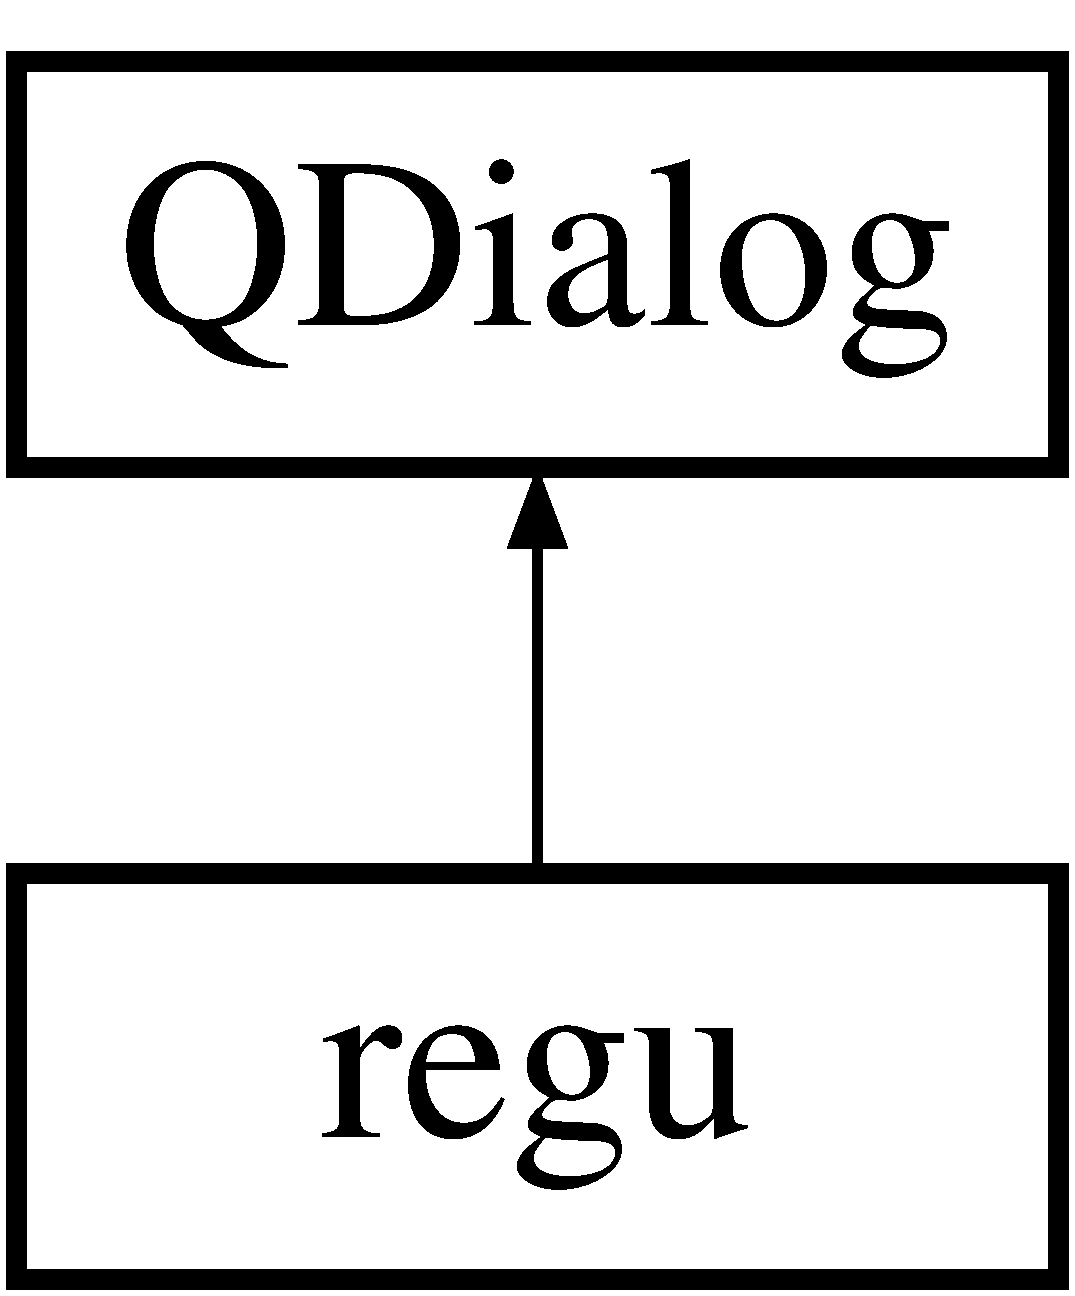
\includegraphics[height=2.000000cm]{classregu}
\end{center}
\end{figure}
\subsection*{Public Member Functions}
\begin{DoxyCompactItemize}
\item 
\hyperlink{classregu_a4233920e912063eba919a7031cadc10a}{regu} (Q\+Widget $\ast$parent=0)
\begin{DoxyCompactList}\small\item\em \hyperlink{classregu_a4233920e912063eba919a7031cadc10a}{regu\+::regu} Es la función del constructor que controla lo que pasa al abrirse la ventana. \end{DoxyCompactList}\item 
\hyperlink{classregu_af4ce8301d06b2636e666ac5c9cf46e36}{$\sim$regu} ()
\begin{DoxyCompactList}\small\item\em \hyperlink{classregu_af4ce8301d06b2636e666ac5c9cf46e36}{regu\+::$\sim$regu} Es la función del destructor que controla lo que pasa al cerrarse la ventana. \end{DoxyCompactList}\end{DoxyCompactItemize}
\subsection*{Public Attributes}
\begin{DoxyCompactItemize}
\item 
string \hyperlink{classregu_a22cc21aa95246c8b198c0e43dc932c9b}{user}
\item 
string \hyperlink{classregu_a5293f6cb33494cf1701c643b2ff17b4b}{contra}
\item 
string \hyperlink{classregu_a5f9ec0ff54143b14c6cd04f360c04d2c}{name}
\item 
string \hyperlink{classregu_a676bef339cfb36f368ca41f2089268d1}{lastname}
\item 
string \hyperlink{classregu_ae71ceda1a90a9836dbf263eaa3bf9a84}{fn}
\item 
string \hyperlink{classregu_a3f72e08908b7acc437d924ee9619438b}{doci}
\item 
int \hyperlink{classregu_a6e25f0b6f043c6f8c563e07b557e90be}{ano}
\item 
int \hyperlink{classregu_aa428968b67b0b19475ba8570238a04fd}{mes}
\item 
int \hyperlink{classregu_a224486fd0b438d8c2fa9339e0df2e2d3}{dia}
\item 
int \hyperlink{classregu_a8e1e0b50d736177379adb192386bba2d}{anioac}
\item 
int \hyperlink{classregu_a132dfdf2c854220e77bd72ef8512f0bd}{mesac}
\item 
int \hyperlink{classregu_a744f894213a241d94323fea13158ea46}{diaac}
\item 
int \hyperlink{classregu_aced7d6b844bf254badde988ba1544d4f}{diaactual}
\item 
int \hyperlink{classregu_ae5fe72d4503fe08944e2d439aca203c6}{mesactual}
\item 
int \hyperlink{classregu_a9a71f2940cd6150de74b89f063682ce1}{anioactual}
\item 
int \hyperlink{classregu_a79d9c62c9fc46b699f5985b693525bfb}{aniomenos}
\end{DoxyCompactItemize}


\subsection{Detailed Description}
Esta clase denominada regu maneja la conexión con la ventana de dialogo donde se registran los datos de un usuario nuevo. 

\subsection{Constructor \& Destructor Documentation}
\mbox{\Hypertarget{classregu_a4233920e912063eba919a7031cadc10a}\label{classregu_a4233920e912063eba919a7031cadc10a}} 
\index{regu@{regu}!regu@{regu}}
\index{regu@{regu}!regu@{regu}}
\subsubsection{\texorpdfstring{regu()}{regu()}}
{\footnotesize\ttfamily regu\+::regu (\begin{DoxyParamCaption}\item[{Q\+Widget $\ast$}]{parent = {\ttfamily 0} }\end{DoxyParamCaption})\hspace{0.3cm}{\ttfamily [explicit]}}



\hyperlink{classregu_a4233920e912063eba919a7031cadc10a}{regu\+::regu} Es la función del constructor que controla lo que pasa al abrirse la ventana. 

EL constructor de la clase.


\begin{DoxyParams}{Parameters}
{\em parent} & Es un puntero tipo Q\+Widget. \\
\hline
\end{DoxyParams}
\mbox{\Hypertarget{classregu_af4ce8301d06b2636e666ac5c9cf46e36}\label{classregu_af4ce8301d06b2636e666ac5c9cf46e36}} 
\index{regu@{regu}!````~regu@{$\sim$regu}}
\index{````~regu@{$\sim$regu}!regu@{regu}}
\subsubsection{\texorpdfstring{$\sim$regu()}{~regu()}}
{\footnotesize\ttfamily regu\+::$\sim$regu (\begin{DoxyParamCaption}{ }\end{DoxyParamCaption})}



\hyperlink{classregu_af4ce8301d06b2636e666ac5c9cf46e36}{regu\+::$\sim$regu} Es la función del destructor que controla lo que pasa al cerrarse la ventana. 

EL destructor de la clase. 

\subsection{Member Data Documentation}
\mbox{\Hypertarget{classregu_a8e1e0b50d736177379adb192386bba2d}\label{classregu_a8e1e0b50d736177379adb192386bba2d}} 
\index{regu@{regu}!anioac@{anioac}}
\index{anioac@{anioac}!regu@{regu}}
\subsubsection{\texorpdfstring{anioac}{anioac}}
{\footnotesize\ttfamily int regu\+::anioac}

Es una variable que guarda el año actual dado por el sistema . \mbox{\Hypertarget{classregu_a9a71f2940cd6150de74b89f063682ce1}\label{classregu_a9a71f2940cd6150de74b89f063682ce1}} 
\index{regu@{regu}!anioactual@{anioactual}}
\index{anioactual@{anioactual}!regu@{regu}}
\subsubsection{\texorpdfstring{anioactual}{anioactual}}
{\footnotesize\ttfamily int regu\+::anioactual}

Es una variable que almacena el valor real del año actual arrojado por el sistema. \mbox{\Hypertarget{classregu_a79d9c62c9fc46b699f5985b693525bfb}\label{classregu_a79d9c62c9fc46b699f5985b693525bfb}} 
\index{regu@{regu}!aniomenos@{aniomenos}}
\index{aniomenos@{aniomenos}!regu@{regu}}
\subsubsection{\texorpdfstring{aniomenos}{aniomenos}}
{\footnotesize\ttfamily int regu\+::aniomenos}

En esta variable se almacena el valor del año de nacimiento ingresado por el paciente y le suma uno para futuros calculos \mbox{\Hypertarget{classregu_a6e25f0b6f043c6f8c563e07b557e90be}\label{classregu_a6e25f0b6f043c6f8c563e07b557e90be}} 
\index{regu@{regu}!ano@{ano}}
\index{ano@{ano}!regu@{regu}}
\subsubsection{\texorpdfstring{ano}{ano}}
{\footnotesize\ttfamily int regu\+::ano}

Es una variable que guarda el año de nacimiento del paciente que fue ingresado. \mbox{\Hypertarget{classregu_a5293f6cb33494cf1701c643b2ff17b4b}\label{classregu_a5293f6cb33494cf1701c643b2ff17b4b}} 
\index{regu@{regu}!contra@{contra}}
\index{contra@{contra}!regu@{regu}}
\subsubsection{\texorpdfstring{contra}{contra}}
{\footnotesize\ttfamily string regu\+::contra}

Es una variable que guarda la contraseña del usuario. \mbox{\Hypertarget{classregu_a224486fd0b438d8c2fa9339e0df2e2d3}\label{classregu_a224486fd0b438d8c2fa9339e0df2e2d3}} 
\index{regu@{regu}!dia@{dia}}
\index{dia@{dia}!regu@{regu}}
\subsubsection{\texorpdfstring{dia}{dia}}
{\footnotesize\ttfamily int regu\+::dia}

Es una variable que guarda el dia de nacimiento del paciente. \mbox{\Hypertarget{classregu_a744f894213a241d94323fea13158ea46}\label{classregu_a744f894213a241d94323fea13158ea46}} 
\index{regu@{regu}!diaac@{diaac}}
\index{diaac@{diaac}!regu@{regu}}
\subsubsection{\texorpdfstring{diaac}{diaac}}
{\footnotesize\ttfamily int regu\+::diaac}

Es una variable que guarda el dia actual dado por el sistema. \mbox{\Hypertarget{classregu_aced7d6b844bf254badde988ba1544d4f}\label{classregu_aced7d6b844bf254badde988ba1544d4f}} 
\index{regu@{regu}!diaactual@{diaactual}}
\index{diaactual@{diaactual}!regu@{regu}}
\subsubsection{\texorpdfstring{diaactual}{diaactual}}
{\footnotesize\ttfamily int regu\+::diaactual}

Es una variable que almacena el valor real del dia actual arrojado por el sistema. \mbox{\Hypertarget{classregu_a3f72e08908b7acc437d924ee9619438b}\label{classregu_a3f72e08908b7acc437d924ee9619438b}} 
\index{regu@{regu}!doci@{doci}}
\index{doci@{doci}!regu@{regu}}
\subsubsection{\texorpdfstring{doci}{doci}}
{\footnotesize\ttfamily string regu\+::doci}

Es una variable que guarda el documento de identidad del usuario. \mbox{\Hypertarget{classregu_ae71ceda1a90a9836dbf263eaa3bf9a84}\label{classregu_ae71ceda1a90a9836dbf263eaa3bf9a84}} 
\index{regu@{regu}!fn@{fn}}
\index{fn@{fn}!regu@{regu}}
\subsubsection{\texorpdfstring{fn}{fn}}
{\footnotesize\ttfamily string regu\+::fn}

Es una variable que guarda la fecha de nacimiento del usuario, almacenando los dias, el mes y el año, ingresados. \mbox{\Hypertarget{classregu_a676bef339cfb36f368ca41f2089268d1}\label{classregu_a676bef339cfb36f368ca41f2089268d1}} 
\index{regu@{regu}!lastname@{lastname}}
\index{lastname@{lastname}!regu@{regu}}
\subsubsection{\texorpdfstring{lastname}{lastname}}
{\footnotesize\ttfamily string regu\+::lastname}

Es una variable que guarda el apellido del usuario. \mbox{\Hypertarget{classregu_aa428968b67b0b19475ba8570238a04fd}\label{classregu_aa428968b67b0b19475ba8570238a04fd}} 
\index{regu@{regu}!mes@{mes}}
\index{mes@{mes}!regu@{regu}}
\subsubsection{\texorpdfstring{mes}{mes}}
{\footnotesize\ttfamily int regu\+::mes}

Es una variable que guarda el mes de nacimiento del paciente. \mbox{\Hypertarget{classregu_a132dfdf2c854220e77bd72ef8512f0bd}\label{classregu_a132dfdf2c854220e77bd72ef8512f0bd}} 
\index{regu@{regu}!mesac@{mesac}}
\index{mesac@{mesac}!regu@{regu}}
\subsubsection{\texorpdfstring{mesac}{mesac}}
{\footnotesize\ttfamily int regu\+::mesac}

Es una variable que guarda el mes actual dado por el sistema. \mbox{\Hypertarget{classregu_ae5fe72d4503fe08944e2d439aca203c6}\label{classregu_ae5fe72d4503fe08944e2d439aca203c6}} 
\index{regu@{regu}!mesactual@{mesactual}}
\index{mesactual@{mesactual}!regu@{regu}}
\subsubsection{\texorpdfstring{mesactual}{mesactual}}
{\footnotesize\ttfamily int regu\+::mesactual}

Es una variable que almacena el valor real del mes actual arrojado por el sistema. \mbox{\Hypertarget{classregu_a5f9ec0ff54143b14c6cd04f360c04d2c}\label{classregu_a5f9ec0ff54143b14c6cd04f360c04d2c}} 
\index{regu@{regu}!name@{name}}
\index{name@{name}!regu@{regu}}
\subsubsection{\texorpdfstring{name}{name}}
{\footnotesize\ttfamily string regu\+::name}

Es una variable que guarda el nombre del usuario. \mbox{\Hypertarget{classregu_a22cc21aa95246c8b198c0e43dc932c9b}\label{classregu_a22cc21aa95246c8b198c0e43dc932c9b}} 
\index{regu@{regu}!user@{user}}
\index{user@{user}!regu@{regu}}
\subsubsection{\texorpdfstring{user}{user}}
{\footnotesize\ttfamily string regu\+::user}

Es una variable que guarda el nickname del usuario. 

The documentation for this class was generated from the following files\+:\begin{DoxyCompactItemize}
\item 
/home/alseuser/\+Proecto\+\_\+final\+\_\+alse/\+P\+A/regu.\+h\item 
/home/alseuser/\+Proecto\+\_\+final\+\_\+alse/\+P\+A/regu.\+cpp\end{DoxyCompactItemize}

\hypertarget{classtiempod}{}\section{tiempod Class Reference}
\label{classtiempod}\index{tiempod@{tiempod}}


Esta clase maneja la conexion con al ventana donde le preguntaremos al usuario la duracion de la prueba de agilidad para el paciente.  




{\ttfamily \#include $<$tiempod.\+h$>$}

Inheritance diagram for tiempod\+:\begin{figure}[H]
\begin{center}
\leavevmode
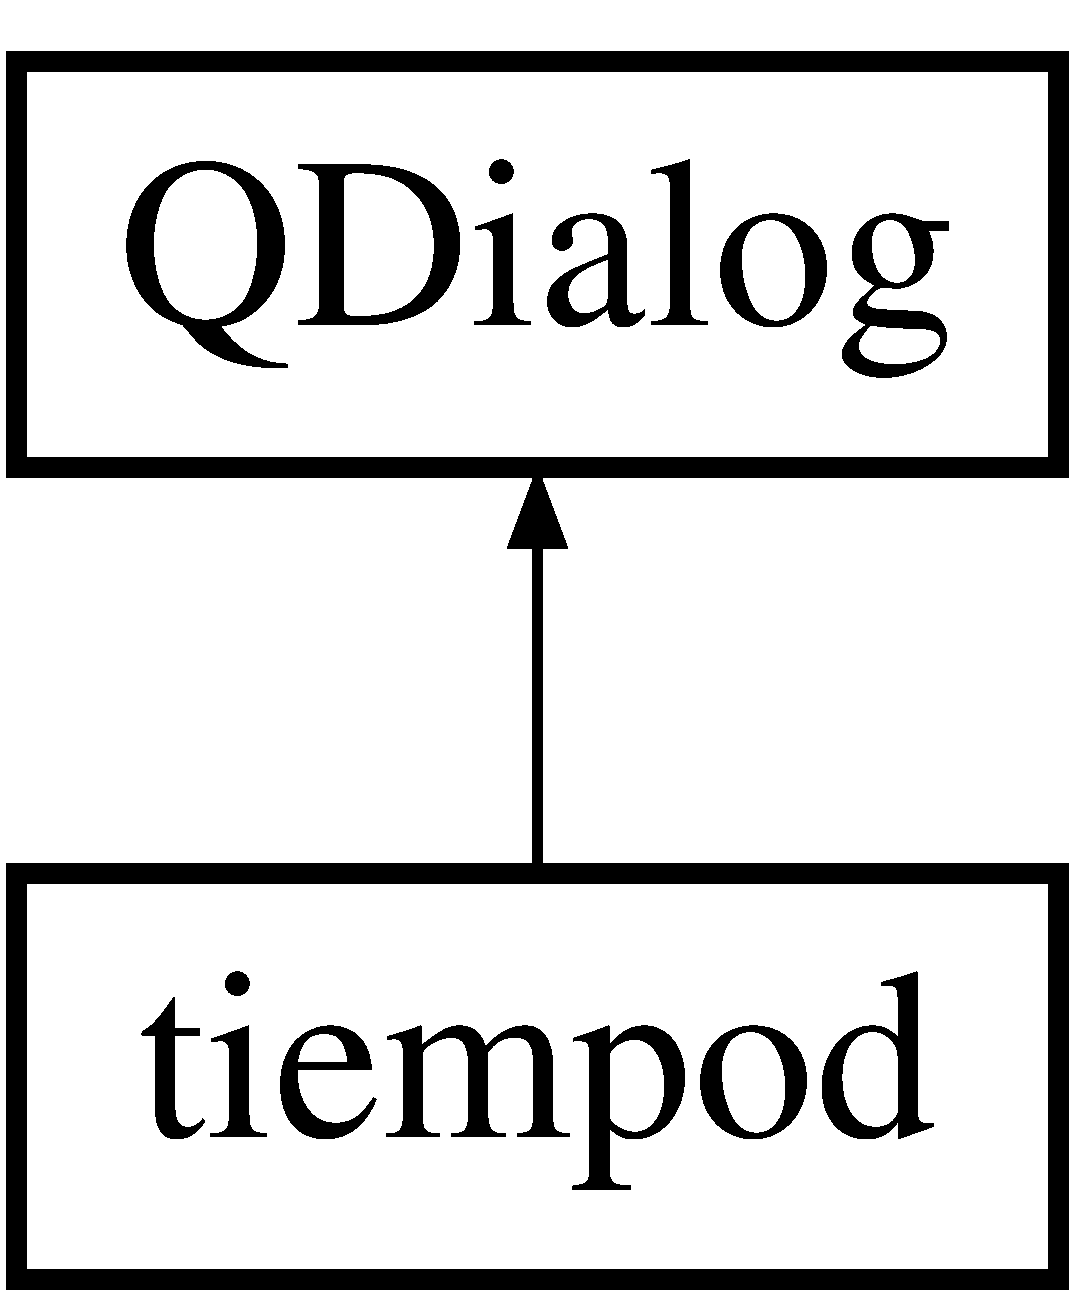
\includegraphics[height=2.000000cm]{classtiempod}
\end{center}
\end{figure}
\subsection*{Public Member Functions}
\begin{DoxyCompactItemize}
\item 
\hyperlink{classtiempod_a0c0071faff0c83839d6bdecdbef92e6e}{tiempod} (Q\+Widget $\ast$parent=0)
\begin{DoxyCompactList}\small\item\em \hyperlink{classtiempod_a0c0071faff0c83839d6bdecdbef92e6e}{tiempod\+::tiempod} Es la funcion del constructor que controla lo que pasa al abrirse la ventana. \end{DoxyCompactList}\item 
\hyperlink{classtiempod_a5107437d6cac97c1b63c3ff9df5a9e36}{$\sim$tiempod} ()
\begin{DoxyCompactList}\small\item\em \hyperlink{classtiempod_a5107437d6cac97c1b63c3ff9df5a9e36}{tiempod\+::$\sim$tiempod} Es la funcion del destructor que controla lo que pasa al cerrarse la ventana. \end{DoxyCompactList}\end{DoxyCompactItemize}


\subsection{Detailed Description}
Esta clase maneja la conexion con al ventana donde le preguntaremos al usuario la duracion de la prueba de agilidad para el paciente. 

\subsection{Constructor \& Destructor Documentation}
\mbox{\Hypertarget{classtiempod_a0c0071faff0c83839d6bdecdbef92e6e}\label{classtiempod_a0c0071faff0c83839d6bdecdbef92e6e}} 
\index{tiempod@{tiempod}!tiempod@{tiempod}}
\index{tiempod@{tiempod}!tiempod@{tiempod}}
\subsubsection{\texorpdfstring{tiempod()}{tiempod()}}
{\footnotesize\ttfamily tiempod\+::tiempod (\begin{DoxyParamCaption}\item[{Q\+Widget $\ast$}]{parent = {\ttfamily 0} }\end{DoxyParamCaption})\hspace{0.3cm}{\ttfamily [explicit]}}



\hyperlink{classtiempod_a0c0071faff0c83839d6bdecdbef92e6e}{tiempod\+::tiempod} Es la funcion del constructor que controla lo que pasa al abrirse la ventana. 

EL constructor de la clase.


\begin{DoxyParams}{Parameters}
{\em parent} & es un puntero tipo Q\+Widget. \\
\hline
\end{DoxyParams}
\mbox{\Hypertarget{classtiempod_a5107437d6cac97c1b63c3ff9df5a9e36}\label{classtiempod_a5107437d6cac97c1b63c3ff9df5a9e36}} 
\index{tiempod@{tiempod}!````~tiempod@{$\sim$tiempod}}
\index{````~tiempod@{$\sim$tiempod}!tiempod@{tiempod}}
\subsubsection{\texorpdfstring{$\sim$tiempod()}{~tiempod()}}
{\footnotesize\ttfamily tiempod\+::$\sim$tiempod (\begin{DoxyParamCaption}{ }\end{DoxyParamCaption})}



\hyperlink{classtiempod_a5107437d6cac97c1b63c3ff9df5a9e36}{tiempod\+::$\sim$tiempod} Es la funcion del destructor que controla lo que pasa al cerrarse la ventana. 

EL destructor de la clase. 

The documentation for this class was generated from the following files\+:\begin{DoxyCompactItemize}
\item 
/home/alseuser/\+Proecto\+\_\+final\+\_\+alse/\+P\+A/tiempod.\+h\item 
/home/alseuser/\+Proecto\+\_\+final\+\_\+alse/\+P\+A/tiempod.\+cpp\end{DoxyCompactItemize}

\hypertarget{classusuario}{}\section{usuario Class Reference}
\label{classusuario}\index{usuario@{usuario}}


esta clase maneja la verificacion de usuario que se realiza en la ventana principal.  




{\ttfamily \#include $<$usuario.\+h$>$}

Inheritance diagram for usuario\+:\begin{figure}[H]
\begin{center}
\leavevmode
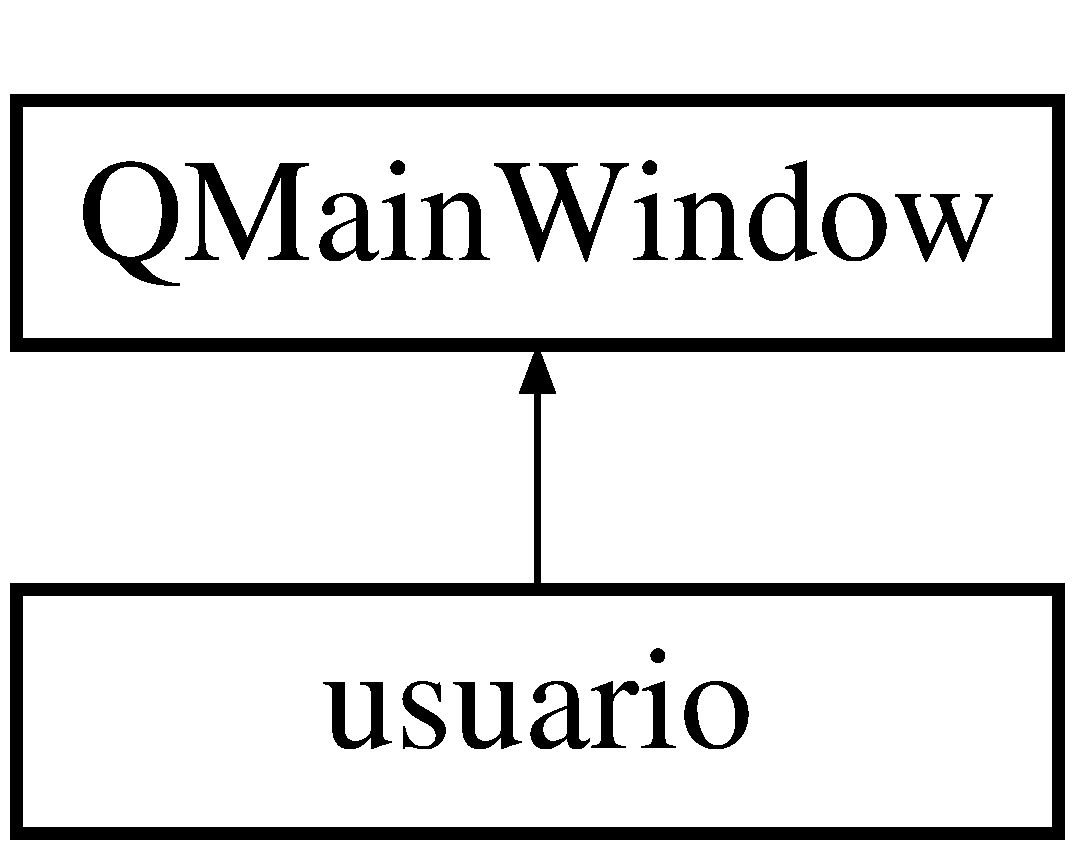
\includegraphics[height=2.000000cm]{classusuario}
\end{center}
\end{figure}
\subsection*{Public Member Functions}
\begin{DoxyCompactItemize}
\item 
\hyperlink{classusuario_a34821186e90424c9105221fb931e9ca0}{usuario} (Q\+Widget $\ast$parent=0)
\begin{DoxyCompactList}\small\item\em \hyperlink{classusuario_a34821186e90424c9105221fb931e9ca0}{usuario\+::usuario} Es la función del constructor que controla lo que pasa al abrirse la ventana. \end{DoxyCompactList}\item 
\hyperlink{classusuario_aa70d0ad5fba6586c37b429b1806ff672}{$\sim$usuario} ()
\begin{DoxyCompactList}\small\item\em \hyperlink{classusuario_aa70d0ad5fba6586c37b429b1806ff672}{usuario\+::$\sim$usuario} Es la función del destructor que controla lo que pasa al cerrarse la ventana. \end{DoxyCompactList}\item 
string \hyperlink{classusuario_a0a32493a53b4aed9d66662f8e6839889}{get\+User} () const
\begin{DoxyCompactList}\small\item\em \hyperlink{classusuario_a0a32493a53b4aed9d66662f8e6839889}{usuario\+::get\+User} \end{DoxyCompactList}\item 
void \hyperlink{classusuario_a0dc83a4f7544e487109854604f167e94}{set\+User} (const string \&value)
\begin{DoxyCompactList}\small\item\em \hyperlink{classusuario_a0dc83a4f7544e487109854604f167e94}{usuario\+::set\+User} \end{DoxyCompactList}\item 
string \hyperlink{classusuario_ae8abb797a4efda6053b2c15936ba9792}{get\+Contra} () const
\begin{DoxyCompactList}\small\item\em \hyperlink{classusuario_ae8abb797a4efda6053b2c15936ba9792}{usuario\+::get\+Contra()} \end{DoxyCompactList}\item 
void \hyperlink{classusuario_a8e027d694579ff05152cc77c50886111}{set\+Contra} (const string \&value)
\begin{DoxyCompactList}\small\item\em \hyperlink{classusuario_a8e027d694579ff05152cc77c50886111}{usuario\+::set\+Contra} \end{DoxyCompactList}\end{DoxyCompactItemize}


\subsection{Detailed Description}
esta clase maneja la verificacion de usuario que se realiza en la ventana principal. 

\subsection{Constructor \& Destructor Documentation}
\mbox{\Hypertarget{classusuario_a34821186e90424c9105221fb931e9ca0}\label{classusuario_a34821186e90424c9105221fb931e9ca0}} 
\index{usuario@{usuario}!usuario@{usuario}}
\index{usuario@{usuario}!usuario@{usuario}}
\subsubsection{\texorpdfstring{usuario()}{usuario()}}
{\footnotesize\ttfamily usuario\+::usuario (\begin{DoxyParamCaption}\item[{Q\+Widget $\ast$}]{parent = {\ttfamily 0} }\end{DoxyParamCaption})\hspace{0.3cm}{\ttfamily [explicit]}}



\hyperlink{classusuario_a34821186e90424c9105221fb931e9ca0}{usuario\+::usuario} Es la función del constructor que controla lo que pasa al abrirse la ventana. 

EL constructor de la clase.


\begin{DoxyParams}{Parameters}
{\em parent} & Es un puntero tipo Q\+Widget. \\
\hline
\end{DoxyParams}
\mbox{\Hypertarget{classusuario_aa70d0ad5fba6586c37b429b1806ff672}\label{classusuario_aa70d0ad5fba6586c37b429b1806ff672}} 
\index{usuario@{usuario}!````~usuario@{$\sim$usuario}}
\index{````~usuario@{$\sim$usuario}!usuario@{usuario}}
\subsubsection{\texorpdfstring{$\sim$usuario()}{~usuario()}}
{\footnotesize\ttfamily usuario\+::$\sim$usuario (\begin{DoxyParamCaption}{ }\end{DoxyParamCaption})}



\hyperlink{classusuario_aa70d0ad5fba6586c37b429b1806ff672}{usuario\+::$\sim$usuario} Es la función del destructor que controla lo que pasa al cerrarse la ventana. 

EL destructor de la clase. 

\subsection{Member Function Documentation}
\mbox{\Hypertarget{classusuario_ae8abb797a4efda6053b2c15936ba9792}\label{classusuario_ae8abb797a4efda6053b2c15936ba9792}} 
\index{usuario@{usuario}!get\+Contra@{get\+Contra}}
\index{get\+Contra@{get\+Contra}!usuario@{usuario}}
\subsubsection{\texorpdfstring{get\+Contra()}{getContra()}}
{\footnotesize\ttfamily string usuario\+::get\+Contra (\begin{DoxyParamCaption}{ }\end{DoxyParamCaption}) const}



\hyperlink{classusuario_ae8abb797a4efda6053b2c15936ba9792}{usuario\+::get\+Contra()} 

Es la función get de la variable \char`\"{}contra\char`\"{} que recupera o consigue el valor asignado en la función set para ser utilizado después. \begin{DoxyReturn}{Returns}
El valor ingresado en la función set. 
\end{DoxyReturn}
\mbox{\Hypertarget{classusuario_a0a32493a53b4aed9d66662f8e6839889}\label{classusuario_a0a32493a53b4aed9d66662f8e6839889}} 
\index{usuario@{usuario}!get\+User@{get\+User}}
\index{get\+User@{get\+User}!usuario@{usuario}}
\subsubsection{\texorpdfstring{get\+User()}{getUser()}}
{\footnotesize\ttfamily string usuario\+::get\+User (\begin{DoxyParamCaption}{ }\end{DoxyParamCaption}) const}



\hyperlink{classusuario_a0a32493a53b4aed9d66662f8e6839889}{usuario\+::get\+User} 

Es la función get de la variable \char`\"{}user\char`\"{} que recupera o consigue el valor asignado en la función set para ser utilizado después. \begin{DoxyReturn}{Returns}
El valor ingresado en la función set. 
\end{DoxyReturn}
\mbox{\Hypertarget{classusuario_a8e027d694579ff05152cc77c50886111}\label{classusuario_a8e027d694579ff05152cc77c50886111}} 
\index{usuario@{usuario}!set\+Contra@{set\+Contra}}
\index{set\+Contra@{set\+Contra}!usuario@{usuario}}
\subsubsection{\texorpdfstring{set\+Contra()}{setContra()}}
{\footnotesize\ttfamily void usuario\+::set\+Contra (\begin{DoxyParamCaption}\item[{const string \&}]{value }\end{DoxyParamCaption})}



\hyperlink{classusuario_a8e027d694579ff05152cc77c50886111}{usuario\+::set\+Contra} 

Es la función set de la variable \char`\"{}contra\char`\"{} que nos permite darle un valor a esta. 
\begin{DoxyParams}{Parameters}
{\em value} & Es un puntero tipo string. \\
\hline
\end{DoxyParams}
\mbox{\Hypertarget{classusuario_a0dc83a4f7544e487109854604f167e94}\label{classusuario_a0dc83a4f7544e487109854604f167e94}} 
\index{usuario@{usuario}!set\+User@{set\+User}}
\index{set\+User@{set\+User}!usuario@{usuario}}
\subsubsection{\texorpdfstring{set\+User()}{setUser()}}
{\footnotesize\ttfamily void usuario\+::set\+User (\begin{DoxyParamCaption}\item[{const string \&}]{value }\end{DoxyParamCaption})}



\hyperlink{classusuario_a0dc83a4f7544e487109854604f167e94}{usuario\+::set\+User} 

Es la función set de la variable \char`\"{}user\char`\"{} que nos permite darle un valor a esta. 
\begin{DoxyParams}{Parameters}
{\em value} & Es un puntero tipo string. \\
\hline
\end{DoxyParams}


The documentation for this class was generated from the following files\+:\begin{DoxyCompactItemize}
\item 
/home/alseuser/\+Proecto\+\_\+final\+\_\+alse/\+P\+A/usuario.\+h\item 
/home/alseuser/\+Proecto\+\_\+final\+\_\+alse/\+P\+A/usuario.\+cpp\end{DoxyCompactItemize}

%--- End generated contents ---

% Index
\backmatter
\newpage
\phantomsection
\clearemptydoublepage
\addcontentsline{toc}{chapter}{Index}
\printindex

\end{document}
